\documentclass[12pt, a4paper]{article}

% --- KHAI BÁO TIẾNG VIỆT & PHÔNG CHỮ ---
\usepackage[utf8]{inputenc}
\usepackage[T5]{fontenc}
\usepackage[vietnamese]{babel}

% --- CÁC GÓI TOÁN HỌC & ĐỊNH DẠNG HỌC THUẬT ---
\usepackage{amsmath, amssymb, amsthm}
\usepackage{graphicx}
\usepackage{booktabs}
\usepackage{tabularx}
\usepackage{array}
\usepackage{float}
\usepackage{geometry}
\geometry{a4paper, top=2.2cm, bottom=2.0cm, left=2.2cm, right=2.0cm}
\usepackage{fancyhdr}
\usepackage{tikz}
\usetikzlibrary{calc}
\usepackage{xcolor}
\usepackage{hyperref}
\usepackage{cite}

\definecolor{hcmutnavy}{RGB}{0,0,128}

\hypersetup{
    colorlinks=true,
    linkcolor=black,
    citecolor=blue,
    urlcolor=blue
}

% --- TIÊU ĐỀ ĐẦU TRANG / CHÂN TRANG GIỐNG MẪU BTL1 ---
\pagestyle{fancy}
\fancyhf{}
\fancyhead[L]{\small THÔNG TIN DI ĐỘNG}
\fancyhead[R]{\small Tối ưu Beamforming MU-MISO bằng Heuristic/Tiến hóa}
\fancyfoot[C]{\thepage}
\renewcommand{\headrulewidth}{0pt}
\renewcommand{\footrulewidth}{0pt}

\begin{document}

% =========================================================================
% TRANG BÌA (THEO MẪU ĐH BÁCH KHOA TP.HCM - BTL1 NHÓM 10)
% =========================================================================
\begin{titlepage}
\thispagestyle{empty}

% Khung viền xanh navy (#000080) + viền đen góc vuông lồng ghép kiểu Bách Khoa
\begin{tikzpicture}[remember picture, overlay]
    % Viền trong màu xanh navy dày
    \draw[color=hcmutnavy, line width=4.8pt]
        ($(current page.north west)+(10.6mm,-10.6mm)$) rectangle
        ($(current page.south east)+(-10.6mm,10.6mm)$);

    % Viền ngoài màu đen góc vuông lồng ghép (Greek-key corner meander)
    \draw[color=black, line width=1.05pt]
        % Góc trên-trái
        ($(current page.north west)+(8.5mm,-14.0mm)$) --
        ($(current page.north west)+(12.6mm,-14.0mm)$) --
        ($(current page.north west)+(12.6mm,-8.5mm)$) --
        ($(current page.north west)+(8.5mm,-8.5mm)$) --
        ($(current page.north west)+(8.5mm,-12.6mm)$) --
        ($(current page.north west)+(14.0mm,-12.6mm)$) --
        ($(current page.north west)+(14.0mm,-8.5mm)$) --
        % Cạnh trên -> Góc trên-phải
        ($(current page.north east)+(-14.0mm,-8.5mm)$) --
        ($(current page.north east)+(-14.0mm,-12.6mm)$) --
        ($(current page.north east)+(-8.5mm,-12.6mm)$) --
        ($(current page.north east)+(-8.5mm,-8.5mm)$) --
        ($(current page.north east)+(-12.6mm,-8.5mm)$) --
        ($(current page.north east)+(-12.6mm,-14.0mm)$) --
        ($(current page.north east)+(-8.5mm,-14.0mm)$) --
        % Cạnh phải -> Góc dưới-phải
        ($(current page.south east)+(-8.5mm,14.0mm)$) --
        ($(current page.south east)+(-12.6mm,14.0mm)$) --
        ($(current page.south east)+(-12.6mm,8.5mm)$) --
        ($(current page.south east)+(-8.5mm,8.5mm)$) --
        ($(current page.south east)+(-8.5mm,12.6mm)$) --
        ($(current page.south east)+(-14.0mm,12.6mm)$) --
        ($(current page.south east)+(-14.0mm,8.5mm)$) --
        % Cạnh dưới -> Góc dưới-trái
        ($(current page.south west)+(14.0mm,8.5mm)$) --
        ($(current page.south west)+(14.0mm,12.6mm)$) --
        ($(current page.south west)+(8.5mm,12.6mm)$) --
        ($(current page.south west)+(8.5mm,8.5mm)$) --
        ($(current page.south west)+(12.6mm,8.5mm)$) --
        ($(current page.south west)+(12.6mm,14.0mm)$) --
        ($(current page.south west)+(8.5mm,14.0mm)$) -- cycle;
\end{tikzpicture}

\centering
\vspace*{0.7cm}

{\fontsize{16.5}{22}\selectfont\bfseries ĐẠI HỌC QUỐC GIA TP. HỒ CHÍ MINH\\[0.3em]
TRƯỜNG ĐẠI HỌC BÁCH KHOA\par}

\vspace{1.0cm}

\includegraphics[width=4.5cm]{assets/hcmut_logo.png}
\vspace{0.8cm}

{\fontsize{16.5}{22}\selectfont\bfseries BÁO CÁO BÀI TẬP LỚN 2\par}

\vspace{1.1cm}
{\fontsize{16}{23}\selectfont\bfseries TỐI ƯU BEAMFORMING CHO HỆ THỐNG MU-MISO\\
BẰNG GIẢI THUẬT HEURISTIC / TIẾN HÓA\par}

\vspace{1.1cm}
{\fontsize{13.5}{19}\selectfont\bfseries
Môn Thông tin Di động (EE5019)\\[0.4em]
NHÓM 10 - HK 261\\[0.4em]
Giảng viên hướng dẫn: PGS.TS Hà Hoàng Kha\par}

\vspace{1.0cm}
\renewcommand{\arraystretch}{1.45}
\begin{tabular}{|>{\centering\arraybackslash}p{6.0cm}|>{\centering\arraybackslash}p{5.0cm}|}
    \hline
    \textbf{Sinh viên thực hiện} & \textbf{Mã số sinh viên} \\
    \hline
    Trần Quốc Nam & 2212161 \\
    \hline
    Nguyễn Nhật Quang & 2212746 \\
    \hline
\end{tabular}

\vfill
{\fontsize{12}{15}\selectfont\itshape Thành phố Hồ Chí Minh -- 2026\par}
\vspace{0.6cm}
\end{titlepage}

\pagenumbering{roman}
\tableofcontents
\newpage
\listoffigures
\listoftables
\newpage

\pagenumbering{arabic}
\setcounter{page}{1}

\begin{abstract}
Báo cáo này trình bày việc xây dựng mô hình toán học, thiết kế giải thuật tối ưu và mô phỏng Monte-Carlo bằng Python cho bài toán tạo búp sóng đường xuống (Downlink Transmit Beamforming) trong hệ thống đa người dùng nhiều anten phát -- một anten thu (MU-MISO) trên kênh truyền pha-đinh Rician kèm suy hao đường truyền Log-distance. Bài toán tối đa hóa tổng tốc độ bit (Sum-Rate Maximization) dưới ràng buộc tổng công suất phát của trạm gốc là bài toán tối ưu không lồi và thuộc lớp NP-hard. Chúng tôi triển khai và so sánh ba giải thuật tiến hóa/bầy đàn gồm Differential Evolution (DE), Particle Swarm Optimization (PSO) và Genetic Algorithm (GA) theo hai cơ chế biểu diễn nghiệm: (i) biểu diễn trực tiếp ma trận trọng số phức trong không gian thực $2MK$ chiều kèm chuẩn hóa Frobenius (\texttt{Direct-DE/PSO/GA}), và (ii) biểu diễn theo cấu trúc nghiệm tối ưu đối ngẫu đường lên--đường xuống (\texttt{Struct-DE/PSO/GA}) rút gọn bài toán về $2K$ biến thực độc lập với số anten $M$. Kết quả mô phỏng trung bình trên 100 hiện thực kênh độc lập tại cấu hình $M=8, K=4, P_{\max}=20\,\text{dBm}$ cho thấy \texttt{Struct-DE} đạt 22.68\,bps/Hz, vượt WMMSE (22.22\,bps/Hz), ZF (22.31\,bps/Hz), RZF (20.21\,bps/Hz) và MRT (8.44\,bps/Hz); tại công suất cao $P_{\max}=30\,\text{dBm}$, \texttt{Struct-DE} đạt 34.85\,bps/Hz, cải thiện +281.8\% so với MRT (9.13\,bps/Hz). Báo cáo đồng thời phân tích định lượng hiện tượng lời nguyền số chiều của mã hóa trực tiếp khi $M \to 32$, chế độ quá tải $K > M$, sự hội tụ, độ ổn định thống kê và chi phí tính toán.
\end{abstract}

% =========================================================================
\section{GIỚI THIỆU BÀI TOÁN}
Trong các hệ thống thông tin di động băng rộng hiện đại (4G LTE-Advanced, 5G NR và 6G), kỹ thuật ghép kênh phân chia theo không gian (SDMA) tại trạm gốc nhiều anten cho phép phục vụ đồng thời nhiều người dùng đơn anten trên cùng tài nguyên tần số và thời gian \cite{rappaport2002, tse2005}. Cấu trúc đường xuống này tạo thành hệ thống MU-MISO (Multi-User Multiple-Input Single-Output). Mục tiêu cốt lõi của bộ tạo búp sóng tuyến tính (linear precoder / transmit beamformer) là hướng năng lượng sóng vô tuyến tập trung tới từng người dùng đích đồng thời triệt nhiễu đồng kênh liên người dùng (Multi-User Interference -- MUI).

Các kỹ thuật tạo búp sóng dạng đóng truyền thống như Maximum Ratio Transmission (MRT) \cite{lo1999}, Zero-Forcing (ZF) \cite{spencer2004} và Regularized Zero-Forcing (RZF/MMSE) \cite{peel2005} có độ phức tạp thấp nhưng chưa tối ưu trực tiếp dung lượng tổng trong các điều kiện thực tế (chênh lệch suy hao gần--xa lớn hoặc hệ thống quá tải $K > M$). Trong khi đó, bài toán tối đa hóa tổng tốc độ bit (Sum-Rate Maximization) dưới ràng buộc tổng công suất phát tại trạm gốc có bản chất không lồi và đã được chứng minh là bài toán NP-hard \cite{shi2011, bjornson2014}. Thuật toán lặp Weighted MMSE (WMMSE) \cite{shi2011} cải thiện đáng kể hiệu năng nhưng chỉ đảm bảo hội tụ về điểm dừng KKT cục bộ và có tốc độ hội tụ chậm ở vùng SNR cao khi ma trận kênh kém điều kiện.

Giải thuật tiến hóa và trí tuệ bầy đàn như Differential Evolution (DE) \cite{storn1997}, Particle Swarm Optimization (PSO) \cite{kennedy1995, shi1998} và Genetic Algorithm (GA) \cite{goldberg1989} mở ra hướng tiếp cận tối ưu toàn cục không cần đạo hàm (derivative-free). Trong báo cáo này, chúng tôi xây dựng toàn diện bài toán MU-MISO trên kênh Rician, thiết kế hai cơ chế mã hóa nghiệm cho DE, PSO, GA, triển khai bằng Python vector hóa (kèm bộ kiểm thử tự động \texttt{pytest} + \texttt{hypothesis} và đối chiếu chéo với \texttt{scipy.optimize.differential\_evolution} \cite{virtanen2020}), và đánh giá định lượng trên nhiều kịch bản Monte-Carlo.

% =========================================================================
\section{MÔ HÌNH HỆ THỐNG VÀ MÔ HÌNH KÊNH TRUYỀN}

\subsection{Mô hình tín hiệu hệ thống MU-MISO đường xuống}
Xét một ô mạng microcell 5G NR băng tần n78 hoạt động ở tần số sóng mang $f_c = 3.5\,\text{GHz}$ (bước sóng $\lambda = c / f_c \approx 8.57\,\text{cm}$). Trạm gốc (BS) đặt tại gốc tọa độ $(0, 0)$, trang bị mảng anten thẳng đều (ULA) gồm $M$ phần tử đặt cách nhau nửa bước sóng $d_a = \lambda / 2$, phủ sóng một sector góc $120^\circ$ ($\theta_k \in [-60^\circ, +60^\circ]$) để loại trừ đối xứng gương trước--sau của mảng ULA.

$K$ thiết bị người dùng (UE) đơn anten được sinh ngẫu nhiên phân bố đều theo diện tích trong hình vành khăn có bán kính trong $R_{\min} = 20\,\text{m}$ và bán kính ngoài $R_{\max} = 100\,\text{m}$:
\begin{equation}
    d_k = \sqrt{R_{\min}^2 + u_k (R_{\max}^2 - R_{\min}^2)}, \quad u_k \sim \mathcal{U}(0, 1), \quad \theta_k \sim \mathcal{U}\!\left(-\frac{\pi}{3}, \frac{\pi}{3}\right).
\end{equation}
Tọa độ Descartes của người dùng thứ $k$ là $(x_k, y_k) = (d_k \cos\theta_k, d_k \sin\theta_k)$.

Trạm gốc phát đồng thời vector ký hiệu dữ liệu $\mathbf{s} = [s_1, \dots, s_K]^T \in \mathbb{C}^{K \times 1}$ thỏa mãn $\mathbb{E}[\mathbf{s}\mathbf{s}^H] = \mathbf{I}_K$ qua ma trận tạo búp sóng $\mathbf{W} = [\mathbf{w}_1, \dots, \mathbf{w}_K] \in \mathbb{C}^{M \times K}$. Vector tín hiệu phát tại mảng anten BS là $\mathbf{x} = \sum_{j=1}^{K} \mathbf{w}_j s_j$, và tín hiệu băng gốc thu được tại người dùng $k$ có dạng:
\begin{equation}
    y_k = \underbrace{\mathbf{h}_k^H \mathbf{w}_k s_k}_{\text{Tín hiệu mong muốn}} + \underbrace{\sum_{j \neq k}^{K} \mathbf{h}_k^H \mathbf{w}_j s_j}_{\text{Nhiễu đa người dùng (MUI)}} + n_k, \quad k = 1, \dots, K,
\end{equation}
trong đó $\mathbf{h}_k \in \mathbb{C}^{M \times 1}$ là vector kênh truyền từ BS đến UE $k$, và $n_k \sim \mathcal{CN}(0, \sigma^2)$ là tạp âm trắng Gaussian cộng (AWGN) với công suất $\sigma^2 = -94.0\,\text{dBm}$ (tương ứng băng thông $B = 10\,\text{MHz}$, mật độ phổ tạp âm nhiệt $N_0 = -174\,\text{dBm/Hz}$ và hệ số tạp âm máy thu $\text{NF} = 10\,\text{dB}$).

\subsection{Mô hình suy hao đường truyền và Kênh pha-đinh Rician}
Độ lợi suy hao đường truyền cỡ lớn (Large-scale Path Gain) tuân theo mô hình khoảng cách Log-distance \cite{rappaport2002} với độ lợi không gian tự do Friis tại cự ly tham chiếu $d_0 = 1\,\text{m}$ là $\beta_0 = (\lambda / (4\pi d_0))^2 \approx -43.32\,\text{dB}$:
\begin{equation}
    \beta_k = \beta_0 \left(\frac{d_k}{d_0}\right)^{-\alpha}, \qquad \text{PL}(d_k)\,[\text{dB}] = -10\log_{10}(\beta_0) + 10\alpha \log_{10}\!\left(\frac{d_k}{d_0}\right),
\end{equation}
với hệ số mũ suy hao môi trường microcell đô thị $\alpha = 3.0$.

Kênh truyền pha-đinh cỡ nhỏ được mô hình hóa theo phân bố \textbf{Rician} kết hợp đường truyền tầm nhìn thẳng (LoS) tiền định và thành phần tán xạ đa đường (NLoS) Rayleigh \cite{rappaport2002, tse2005}:
\begin{equation}
    \mathbf{h}_k = \sqrt{\beta_k} \left( \sqrt{\frac{\kappa}{\kappa + 1}} \, \bar{\mathbf{h}}_k^{\text{LoS}} + \sqrt{\frac{1}{\kappa + 1}} \, \tilde{\mathbf{h}}_k^{\text{NLoS}} \right),
\end{equation}
trong đó $\kappa = 10^{K_{\text{dB}}/10}$ là hệ số Rician $K$-factor tuyến tính, $\tilde{\mathbf{h}}_k^{\text{NLoS}} \sim \mathcal{CN}(\mathbf{0}, \mathbf{I}_M)$, và vector đáp ứng mảng ULA cho thành phần LoS là:
\begin{equation}
    \bar{\mathbf{h}}_k^{\text{LoS}} = \left[1, \, e^{j\pi\sin\theta_k}, \, \dots, \, e^{j(M-1)\pi\sin\theta_k}\right]^T \in \mathbb{C}^{M \times 1}.
\end{equation}
Do $\|\bar{\mathbf{h}}_k^{\text{LoS}}\|_2^2 = M$ và $\mathbb{E}[\|\tilde{\mathbf{h}}_k^{\text{NLoS}}\|_2^2] = M$, mô hình bảo toàn chính xác kỳ vọng công suất kênh $\mathbb{E}[\|\mathbf{h}_k\|_2^2] = M\beta_k$.

\subsection{Sơ đồ kiến trúc hệ thống và Các giả thiết mô hình}
Luồng xử lý tín hiệu đường xuống kết hợp vòng lặp tối ưu ma trận tạo búp sóng $\mathbf{W}$ bằng giải thuật heuristic/tiến hóa được tóm tắt trong Hình \ref{fig:arch}. Để bài toán mô phỏng rõ ràng và khả tái lập, hệ thống sử dụng 5 giả thiết cơ bản sau:
\begin{enumerate}
    \item \textbf{Thông tin trạng thái kênh hoàn hảo (Perfect CSI):} Trạm gốc nắm chính xác ma trận kênh $\mathbf{H}$ trong suốt một khối nhất quán kênh (block-fading) để tính toán ma trận $\mathbf{W}$.
    \item \textbf{Kênh pha-đinh phẳng (Flat-fading):} Tín hiệu truyền trong băng hẹp (hoặc xét trên từng sóng mang con OFDM), đáp ứng kênh không thay đổi theo tần số trong thời gian một khe truyền dẫn.
    \item \textbf{Ô mạng đơn tế bào và đồng bộ hoàn hảo:} Không xét nhiễu liên tế bào (inter-cell interference) và giả sử đồng bộ thời gian -- tần số lý tưởng giữa BS và $K$ người dùng.
    \item \textbf{Điều kiện trường xa và mảng ULA lý tưởng:} Khoảng cách tối thiểu $R_{\min} = 20\,\text{m}$ đảm bảo mô hình sóng phẳng trường xa và tránh suy hao kỳ dị gần trạm gốc; các phần tử anten đặt cách đều $\lambda/2$ không xét tương hỗ điện từ (mutual coupling).
    \item \textbf{Nguồn phát độc lập và tạp âm AWGN đồng nhất:} Các ký hiệu dữ liệu $s_k$ độc lập có công suất đơn vị ($\mathbb{E}[\mathbf{s}\mathbf{s}^H] = \mathbf{I}_K$) và mọi người dùng chịu tạp âm nhiệt AWGN cùng phương sai $\sigma^2 = -94.0\,\text{dBm}$.
\end{enumerate}

\begin{figure}[H]
    \centering
    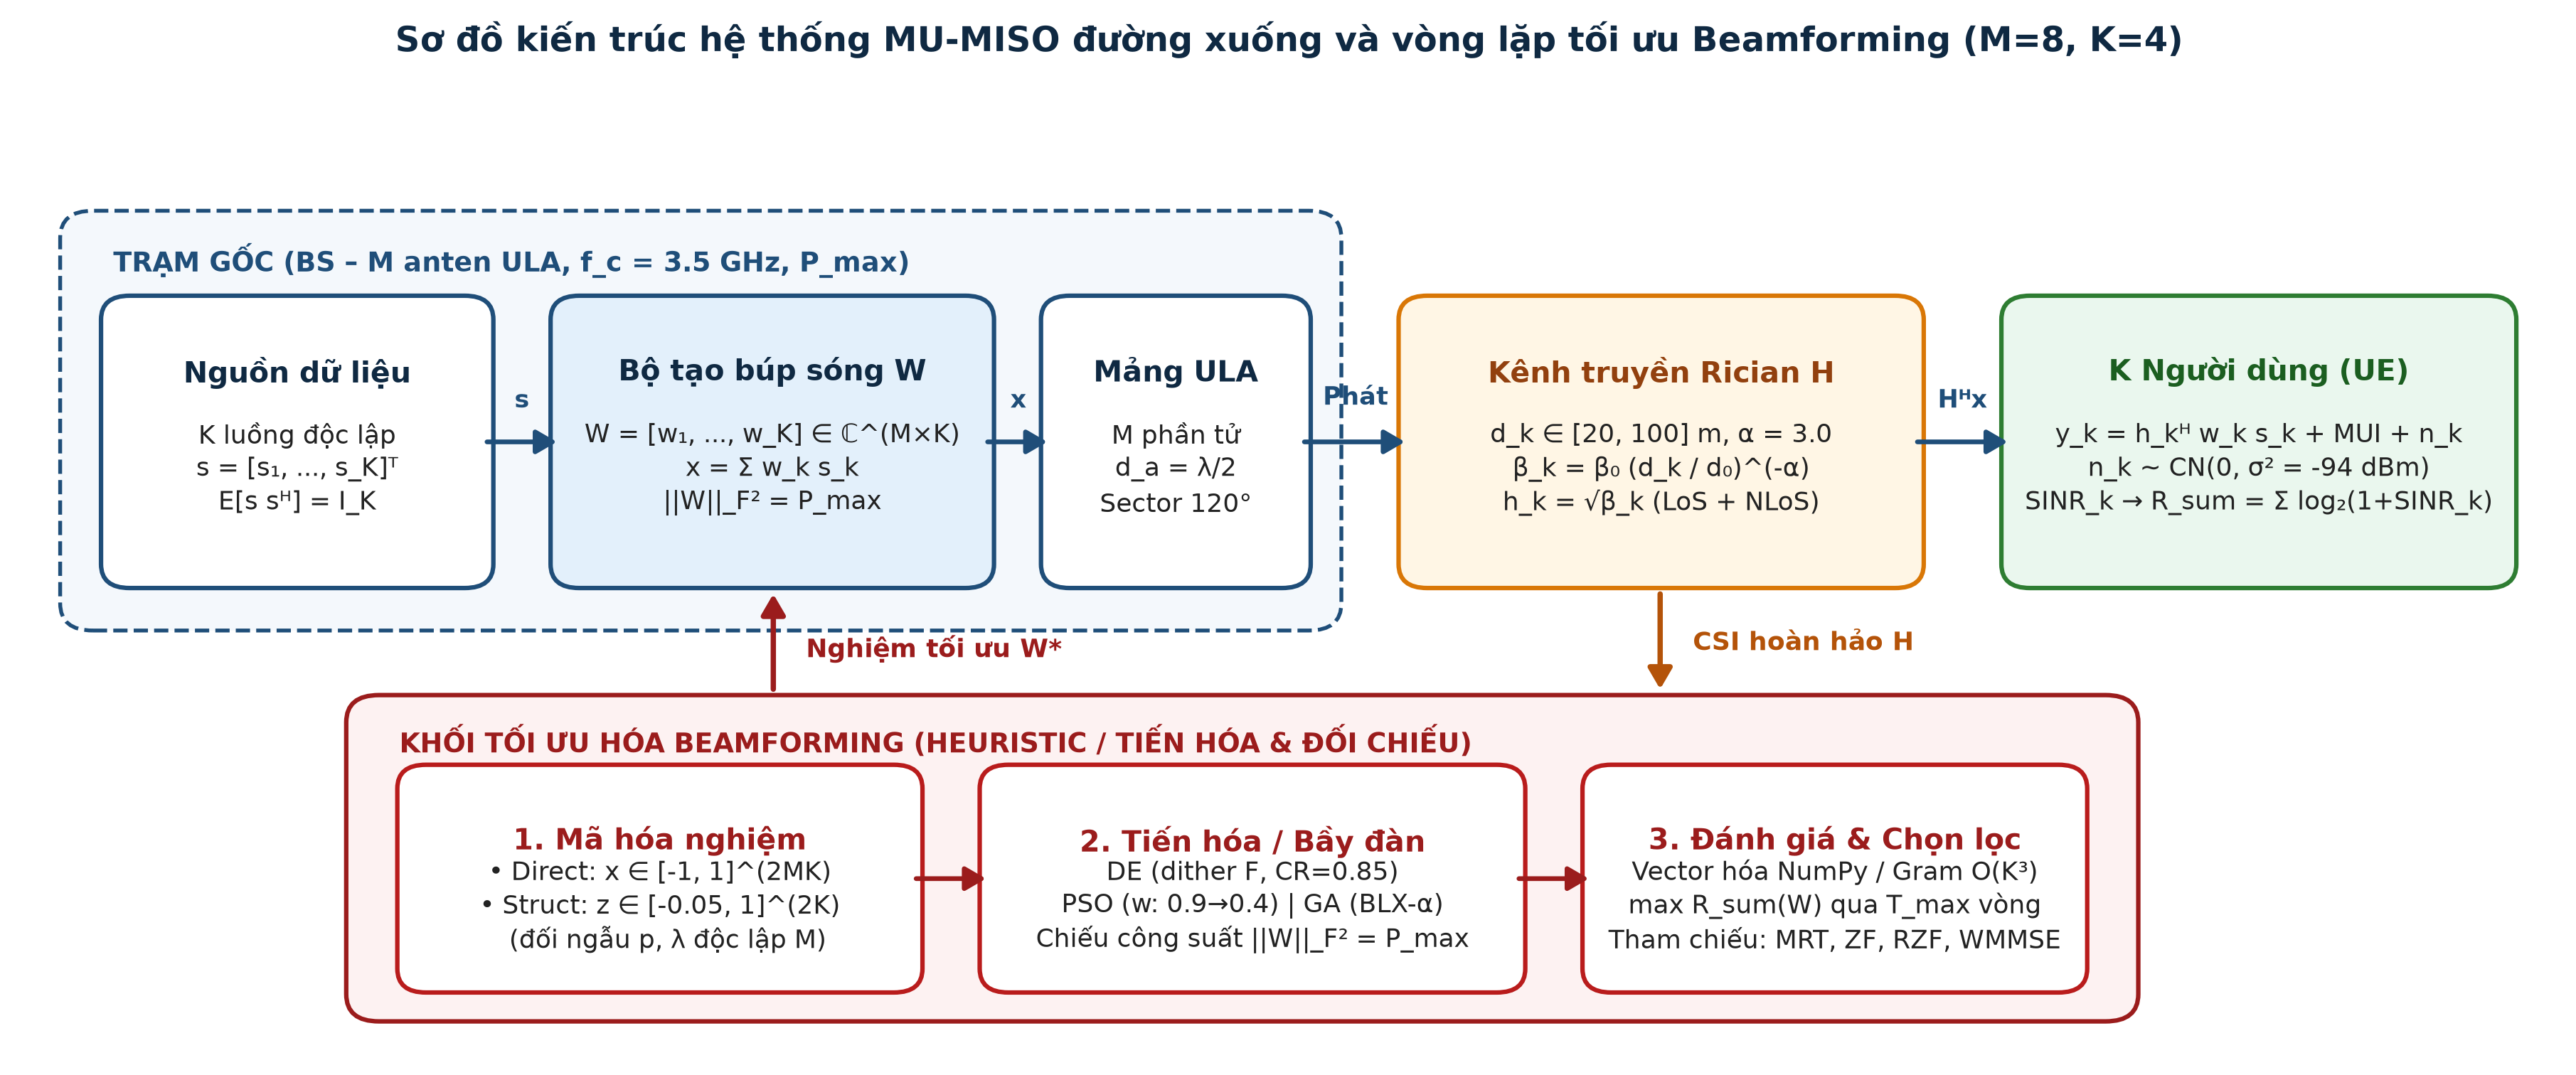
\includegraphics[width=0.98\linewidth]{../results/figures/sodo1_system_architecture.png}
    \caption{Sơ đồ kiến trúc hệ thống MU-MISO đường xuống và vòng lặp tối ưu Beamforming bằng giải thuật Heuristic/Tiến hóa.}
    \label{fig:arch}
\end{figure}

% =========================================================================
\section{XÂY DỰNG BÀI TOÁN TỐI ƯU HÓA}
Tỷ số tín hiệu trên nhiễu cộng tạp âm (SINR) tại người dùng $k$ được xác định bởi:
\begin{equation}
    \text{SINR}_k(\mathbf{W}) = \frac{|\mathbf{h}_k^H \mathbf{w}_k|^2}{\sum_{j \neq k}^{K} |\mathbf{h}_k^H \mathbf{w}_j|^2 + \sigma^2}.
\end{equation}
Theo định lý Shannon, tốc độ bit khả đạt chuẩn hóa theo băng thông của người dùng $k$ là $R_k(\mathbf{W}) = \log_2(1 + \text{SINR}_k(\mathbf{W}))$ (bps/Hz). Bài toán tối đa hóa tổng tốc độ bit dưới ràng buộc tổng công suất phát $P_{\max}$ tại trạm gốc được phát biểu là:
\begin{align}
    (\mathcal{P}1): \quad \max_{\mathbf{W} \in \mathbb{C}^{M \times K}} \quad & R_{\text{sum}}(\mathbf{W}) = \sum_{k=1}^{K} \log_2 \!\left( 1 + \frac{|\mathbf{h}_k^H \mathbf{w}_k|^2}{\sum_{j \neq k}^{K} |\mathbf{h}_k^H \mathbf{w}_j|^2 + \sigma^2} \right) \\
    \text{s.t.} \quad & \sum_{k=1}^{K} \|\mathbf{w}_k\|_2^2 = \|\mathbf{W}\|_F^2 \le P_{\max}.
\end{align}
Hàm mục tiêu $R_{\text{sum}}(\mathbf{W})$ có hai tính chất quan trọng hỗ trợ thiết kế giải thuật: (1) bất biến với phép xoay pha cột $\mathbf{w}_k \mapsto e^{j\phi_k}\mathbf{w}_k$, và (2) tăng chặt theo công suất phát nên nghiệm tối ưu luôn đạt dấu bằng tại biên $\|\mathbf{W}^*\|_F^2 = P_{\max}$.

% =========================================================================
\section{GIẢI THUẬT HEURISTIC / TIẾN HÓA VÀ PHƯƠNG PHÁP THAM CHIẾU}

\subsection{Hai cơ chế biểu diễn nghiệm và xử lý ràng buộc công suất}
\begin{enumerate}
    \item \textbf{Biểu diễn trực tiếp trong không gian $2MK$ chiều (Direct Encoding):} Mỗi cá thể $\mathbf{x} \in [-1, 1]^{2MK}$ ghép nối phần thực và phần ảo của ma trận $\tilde{\mathbf{W}} = \mathbf{X}_{\text{re}} + j\mathbf{X}_{\text{im}} \in \mathbb{C}^{M \times K}$. Ràng buộc tổng công suất được xử lý chính xác không cần hàm phạt thông qua phép chiếu chuẩn hóa Frobenius:
    \begin{equation}
        \mathbf{W} = \sqrt{P_{\max}} \frac{\tilde{\mathbf{W}}}{\|\tilde{\mathbf{W}}\|_F + \varepsilon} \implies \|\mathbf{W}\|_F^2 = P_{\max}.
    \end{equation}
    \item \textbf{Biểu diễn theo cấu trúc nghiệm tối ưu $2K$ chiều (Structure-Guided Encoding):} Để khắc phục sự bùng nổ số chiều $2MK$ khi $M$ lớn, ta khai thác Định lý cấu trúc beamforming đa người dùng tối ưu dựa trên đối ngẫu đường lên--đường xuống \cite{bjornson2014}: mọi nghiệm tối ưu của $(\mathcal{P}1)$ đều có dạng tham số hóa theo công suất đường xuống $p_k \ge 0$ ($\sum_k p_k = P_{\max}$) và trọng số đối ngẫu đường lên $\lambda_k \ge 0$ ($\sum_k \lambda_k = P_{\max}$):
    \begin{equation}
        \mathbf{w}_k(\mathbf{p}, \boldsymbol{\lambda}) = \sqrt{p_k} \frac{\left(\mathbf{I}_M + \sum_{j=1}^{K} \frac{\lambda_j}{\sigma^2}\mathbf{h}_j\mathbf{h}_j^H\right)^{-1}\mathbf{h}_k}{\left\|\left(\mathbf{I}_M + \sum_{j=1}^{K} \frac{\lambda_j}{\sigma^2}\mathbf{h}_j\mathbf{h}_j^H\right)^{-1}\mathbf{h}_k\right\|_2}.
    \end{equation}
    Đặt kênh chuẩn hóa tạp âm $\tilde{\mathbf{H}} = \mathbf{H}/\sqrt{\sigma^2}$ và ma trận Gram $\mathbf{G}_H = \tilde{\mathbf{H}}^H\tilde{\mathbf{H}} \in \mathbb{C}^{K \times K}$. Áp dụng đồng nhất thức đẩy qua (push-through identity):
    \begin{equation}
        \left(\mathbf{I}_M + \tilde{\mathbf{H}}\operatorname{diag}(\boldsymbol{\lambda})\tilde{\mathbf{H}}^H\right)^{-1}\tilde{\mathbf{H}} = \tilde{\mathbf{H}}\left(\mathbf{I}_K + \operatorname{diag}(\boldsymbol{\lambda})\mathbf{G}_H\right)^{-1},
    \end{equation}
    toàn bộ quần thể $\mathbf{Z} \in [-0.05, 1.0]^{N_p \times 2K}$ (cắt ngưỡng $0$ cho phép tự động tắt các UE yếu khi $K > M$) được đánh giá với độ phức tạp chỉ $\mathcal{O}(N_p K^3)$, hoàn toàn độc lập với số anten $M$.
\end{enumerate}

\subsection{Cơ chế hoạt động của DE, PSO và GA}
\begin{itemize}
    \item \textbf{Differential Evolution (DE/current-to-best/1/bin)} \cite{storn1997}: Khởi tạo đều $N_p$ cá thể; mỗi thế hệ tạo vector đột biến $\mathbf{v}_i = \mathbf{x}_i + F_i(\mathbf{x}_{\text{best}} - \mathbf{x}_i) + F_i(\mathbf{x}_{r_1} - \mathbf{x}_{r_2})$ với hệ số dither $F_i \sim \mathcal{U}(0.4, 0.8)$, lai ghép nhị thức xác suất $CR = 0.85$ (luôn chọn tối thiểu 1 tọa độ $j_{\text{rand}}$), kẹp biên và chọn lọc tham lam $\mathbf{x}_i^{(t+1)} = \mathbf{u}_i$ nếu $f(\mathbf{u}_i) \ge f(\mathbf{x}_i^{(t)})$.
    \item \textbf{Particle Swarm Optimization (Global-Best PSO)} \cite{kennedy1995, shi1998}: Cập nhật vận tốc $\mathbf{v}_i^{(t+1)} = w(t)\mathbf{v}_i^{(t)} + c_1 \mathbf{r}_1 \odot (\mathbf{p}_{i,\text{best}} - \mathbf{x}_i^{(t)}) + c_2 \mathbf{r}_2 \odot (\mathbf{g}_{\text{best}} - \mathbf{x}_i^{(t)})$ với trọng số quán tính giảm tuyến tính $w(t): 0.9 \to 0.4$, $c_1 = 1.5, c_2 = 1.8$, kẹp vận tốc $v_{\max} = 0.25 \cdot \text{span}$ và phản xạ tắt dần tại biên.
    \item \textbf{Real-Coded Genetic Algorithm (GA)} \cite{goldberg1989}: Kết hợp chọn lọc đấu loại (Tournament cỡ 3), lai ghép pha trộn BLX-$\alpha$ ($\alpha = 0.3$, $p_c = 0.9$), đột biến Gaussian độ lệch chuẩn giảm tuyến tính ($p_m = 0.12$) và giữ lại 2 cá thể ưu tú (Elitism) nhằm đảm bảo đường cong hội tụ đơn điệu không giảm.
    \item \textbf{Điều kiện dừng và đối chiếu mã nguồn mở:} Mỗi giải thuật dừng khi đạt số thế hệ tối đa $T_{\max} = 250$ với kích thước quần thể $N_p = 50$ ($12.550$ đánh giá) cho biểu diễn trực tiếp $2MK$ chiều, và $T_{\max} = 100$ với $N_p = 36$ ($3.636$ đánh giá) cho biểu diễn cấu trúc $2K$ chiều (đồng thời hỗ trợ cơ chế dừng sớm theo ngưỡng cải thiện $\Delta R < 10^{-6}$ nếu kích hoạt trong \texttt{config.py}). Kết quả \texttt{Struct-DE} được đối chiếu chéo trực tiếp với \texttt{scipy.optimize.differential\_evolution} \cite{virtanen2020} trong bộ kiểm thử tự động.
\end{itemize}

\begin{table}[H]
    \centering
    \caption{Tóm tắt quy trình thực thi giải thuật Differential Evolution (\texttt{Direct-DE} / \texttt{Struct-DE})}
    \label{tab:algo_de}
    \renewcommand{\arraystretch}{1.18}
    \begin{tabularx}{\textwidth}{l X}
        \toprule
        \textbf{Bước} & \textbf{Thao tác trong vòng lặp tiến hóa} \\
        \midrule
        \textbf{Đầu vào} & Ma trận kênh $\mathbf{H} \in \mathbb{C}^{M\times K}$, $P_{\max}$, $\sigma^2$, cỡ quần thể $N_p$, số vòng lặp $T_{\max}$, $F \in [0.4, 0.8]$, $CR = 0.85$. \\
        \textbf{1. Khởi tạo} & Sinh ngẫu nhiên đều $N_p$ cá thể $\mathbf{x}_i^{(0)}$ trong $[-1,1]^{2MK}$ (\texttt{Direct}) hoặc $[-0.05, 1.0]^{2K}$ (\texttt{Struct}); tiền tính ma trận Gram $\mathbf{G}_H = \tilde{\mathbf{H}}^H\tilde{\mathbf{H}}$ nếu dùng \texttt{Struct}. \\
        \textbf{2. Đánh giá đầu} & Chiếu ràng buộc công suất ($\|\mathbf{W}\|_F^2 = P_{\max}$ hoặc $\sum p_k = \sum \lambda_k = P_{\max}$), tính $R_{\text{sum}}$ cho toàn quần thể theo lô và lưu $\mathbf{x}_{\text{best}}$. \\
        \textbf{3. Đột biến \& Lai} & Với mỗi $t = 1 \dots T_{\max}$: tạo $\mathbf{v}_i = \mathbf{x}_i + F_i(\mathbf{x}_{\text{best}} - \mathbf{x}_i) + F_i(\mathbf{x}_{r_1} - \mathbf{x}_{r_2})$, kẹp biên hộp và lai ghép nhị thức theo xác suất $CR$ (đảm bảo tối thiểu một tọa độ $j_{\text{rand}}$) thu được $\mathbf{u}_i$. \\
        \textbf{4. Chọn lọc} & Chuẩn hóa công suất và đánh giá lô $R_{\text{sum}}(\mathbf{u}_i)$; cập nhật $\mathbf{x}_i^{(t)} = \mathbf{u}_i$ nếu $R_{\text{sum}}(\mathbf{u}_i) \ge R_{\text{sum}}(\mathbf{x}_i^{(t-1)})$, ngược lại giữ $\mathbf{x}_i^{(t-1)}$ và cập nhật $\mathbf{x}_{\text{best}}$. \\
        \textbf{5. Dừng \& Xuất} & Dừng khi $t = T_{\max}$; giải mã $\mathbf{x}_{\text{best}}$ thành ma trận $\mathbf{W}^* \in \mathbb{C}^{M \times K}$ thỏa mãn $\|\mathbf{W}^*\|_F^2 = P_{\max}$ và trả về đường cong hội tụ. \\
        \bottomrule
    \end{tabularx}
\end{table}

\subsection{Các phương pháp tham chiếu (Baselines)}
Hiệu năng các giải thuật tiến hóa được đối chiếu trên cùng tập kênh với 4 phương pháp kinh điển:
(1) \textbf{MRT} \cite{lo1999}: $\mathbf{w}_k = \sqrt{P_{\max}/K}\,\mathbf{h}_k/\|\mathbf{h}_k\|_2$;
(2) \textbf{ZF} \cite{spencer2004}: giả nghịch đảo $\mathbf{V} = (\mathbf{H}^H)^\dagger$, chuẩn hóa cột và chia đều công suất;
(3) \textbf{RZF/MMSE} \cite{peel2005}: $\mathbf{V} = \mathbf{H}(\mathbf{H}^H\mathbf{H} + \frac{K\sigma^2}{P_{\max}}\mathbf{I}_K)^{-1}$ chuẩn hóa tổng công suất $P_{\max}$; và
(4) \textbf{WMMSE} \cite{shi2011}: lặp luân phiên cập nhật $u_k$, $\rho_k = 1/e_k$ và giải phương trình Lagrange $\mathbf{W}(\mu) = (\mathbf{A} + \mu\mathbf{I}_M)^{-1}\mathbf{B}$ bằng chia đôi 60 bước trên phân rã trị riêng của $\mathbf{A}$.

% =========================================================================
\section{THIẾT LẬP MÔ PHỎNG VÀ KIỂM THỬ}
Toàn bộ mã nguồn được xây dựng bằng Python với cấu trúc module tách biệt (\texttt{config.py}, \texttt{src/channel.py}, \texttt{src/metrics.py}, \texttt{src/baselines.py}, \texttt{src/optimizers.py}, \texttt{src/experiments.py}), vector hóa hoàn toàn bằng NumPy/SciPy và kiểm chứng tự động bằng bộ 21 kịch bản \texttt{pytest} + \texttt{hypothesis} (kiểm tra thống kê kênh Rician $\mathbb{E}[\|\mathbf{h}_k\|_2^2] \approx M\beta_k$, ràng buộc công suất $\|\mathbf{W}\|_F^2 \le P_{\max}$, tính bất biến pha, triệt nhiễu ZF $< 10^{-10}$, tính đơn điệu hội tụ và đối chiếu chéo với \texttt{scipy.optimize.differential\_evolution} \cite{virtanen2020}).

\subsection{Căn cứ lựa chọn tham số, giải thuật và tiêu chí đánh giá}
\begin{itemize}
    \item \textbf{Lựa chọn tham số hệ thống và kênh truyền:} Tần số $f_c = 3.5\,\text{GHz}$ và băng thông $B = 10\,\text{MHz}$ đại diện cho mạng 5G NR n78 microcell đô thị; công suất tạp âm $\sigma^2 = -174 + 10\log_{10}(10^7) + 10 = -94.0\,\text{dBm}$ kết hợp suy hao Log-distance ($\alpha = 3.0$, $d_k \in [20, 100]\,\text{m}$) giúp dải $P_{\max} \in [0, 30]\,\text{dBm}$ bao phủ trọn vẹn từ miền công suất thấp đến miền giới hạn nhiễu cao. Góc sector $120^\circ$ phù hợp kiến trúc 3 sector thực tế và tránh đối xứng gương trước--sau của mảng ULA; số mẫu $100$ kênh độc lập (với hạt giống cố định \texttt{seed=2026}) và $30$ lần chạy lặp đảm bảo đường cong trung bình mượt và đánh giá được độ phân tán thống kê.
    \item \textbf{Lựa chọn giải thuật tối ưu:} \texttt{DE} được chọn làm giải thuật chủ đạo vì hoạt động vượt trội trên không gian thực liên tục, ít siêu tham số nhạy cảm và toán tử đột biến vi sai thích nghi tự động theo cấu trúc địa hình hàm mục tiêu. Nhóm đồng thời triển khai \texttt{PSO} (đại diện trí tuệ bầy đàn) và \texttt{GA} (đại diện tiến hóa kinh điển) cùng hai cơ chế biểu diễn (\texttt{Direct} $2MK$ và \texttt{Struct} $2K$) để chứng minh định lượng lợi ích của việc kết hợp tri thức vật lý vào giải thuật heuristic, đồng thời đối chiếu với 4 phương pháp tham chiếu (\texttt{MRT}, \texttt{ZF}, \texttt{RZF}, \texttt{WMMSE}) và \texttt{SciPy-DE}.
    \item \textbf{Lựa chọn tiêu chí đánh giá:} Hiệu năng hệ thống được đánh giá toàn diện theo 4 trục: (1) \emph{Tổng tốc độ bit trung bình} [bps/Hz] đo hiệu quả phổ trung bình trên nhiều hiện thực kênh; (2) \emph{Đường cong hội tụ trung bình $\pm 1\sigma$} theo số thế hệ đo tốc độ tiến hóa; (3) \emph{Độ lệch chuẩn (Std) và hệ số biến thiên (CV \%)} qua 30 lần chạy độc lập đo độ ổn định của giải thuật ngẫu nhiên; và (4) \emph{Thời gian thực thi trung bình (ms) cùng số lần đánh giá hàm mục tiêu} đo chi phí tính toán thực tế.
\end{itemize}

\subsection{Bảng tổng hợp tham số mô phỏng}

\begin{table}[H]
    \centering
    \caption{Bảng tổng hợp các tham số hệ thống, kênh truyền và giải thuật mô phỏng}
    \label{tab:params}
    \renewcommand{\arraystretch}{1.2}
    \begin{tabularx}{\textwidth}{l l X}
        \toprule
        \textbf{Tham số} & \textbf{Giá trị} & \textbf{Ghi chú / Ý nghĩa} \\
        \midrule
        Tần số $f_c$ / Băng thông $B$ & 3.5\,GHz / 10\,MHz & Băng tần 5G NR n78 ($\lambda \approx 8.57$\,cm) \\
        Vùng phủ sóng sector ULA & $R \in [20, 100]$\,m, $120^\circ$ & Phân bố đều theo diện tích, khoảng cách anten $\lambda/2$ \\
        Suy hao đường truyền & $\beta_0 \approx -43.32$\,dB, $\alpha = 3.0$ & Log-distance Friis tại $d_0 = 1$\,m \cite{rappaport2002} \\
        Hệ số Rician $K$-factor & $6$\,dB (quét $-20 \dots 15$\,dB) & Kết hợp LoS ULA và tán xạ Rayleigh NLoS \\
        Tạp âm AWGN $\sigma^2$ & $-94.0$\,dBm & $N_0 = -174$\,dBm/Hz, $\text{NF} = 10$\,dB \\
        Cấu hình mặc định & $M=8, K=4, P_{\max}=20$\,dBm & Kịch bản cơ sở cho các khảo sát tham số \\
        Số mẫu Monte-Carlo & 100 kênh / 30 lần ổn định & Hạt giống cố định \texttt{seed=2026} \\
        \texttt{Direct-DE/PSO/GA} & $N_p=50, T_{\max}=250$ & Không gian $2MK$ biến thực (12.550 evals) \\
        \texttt{Struct-DE/PSO/GA} & $N_p=36, T_{\max}=100$ & Không gian $2K$ biến đối ngẫu (3.636 evals) \\
        \bottomrule
    \end{tabularx}
\end{table}

% =========================================================================
\section{KẾT QUẢ MÔ PHỎNG VÀ PHÂN TÍCH ĐỊNH LƯỢNG}

\subsection{Kịch bản phủ sóng và Giản đồ búp sóng ULA}
Hình \ref{fig:geom} minh họa một kịch bản phân bố ngẫu nhiên $K=4$ người dùng trong sector $120^\circ$ (thông số chi tiết tại Bảng \ref{tab:ue}) cùng giản đồ bức xạ góc phương vị của bộ tạo búp sóng \texttt{Struct-DE}. Có thể quan sát rõ từng búp sóng đều tập trung đỉnh chính (mainlobe) vào đúng góc phương vị $\theta_k$ của người dùng đích, đồng thời tạo các hõm suy giảm sâu (null) từ $-15$\,dB đến dưới $-30$\,dB về phía các người dùng gây nhiễu còn lại.

\begin{figure}[H]
    \centering
    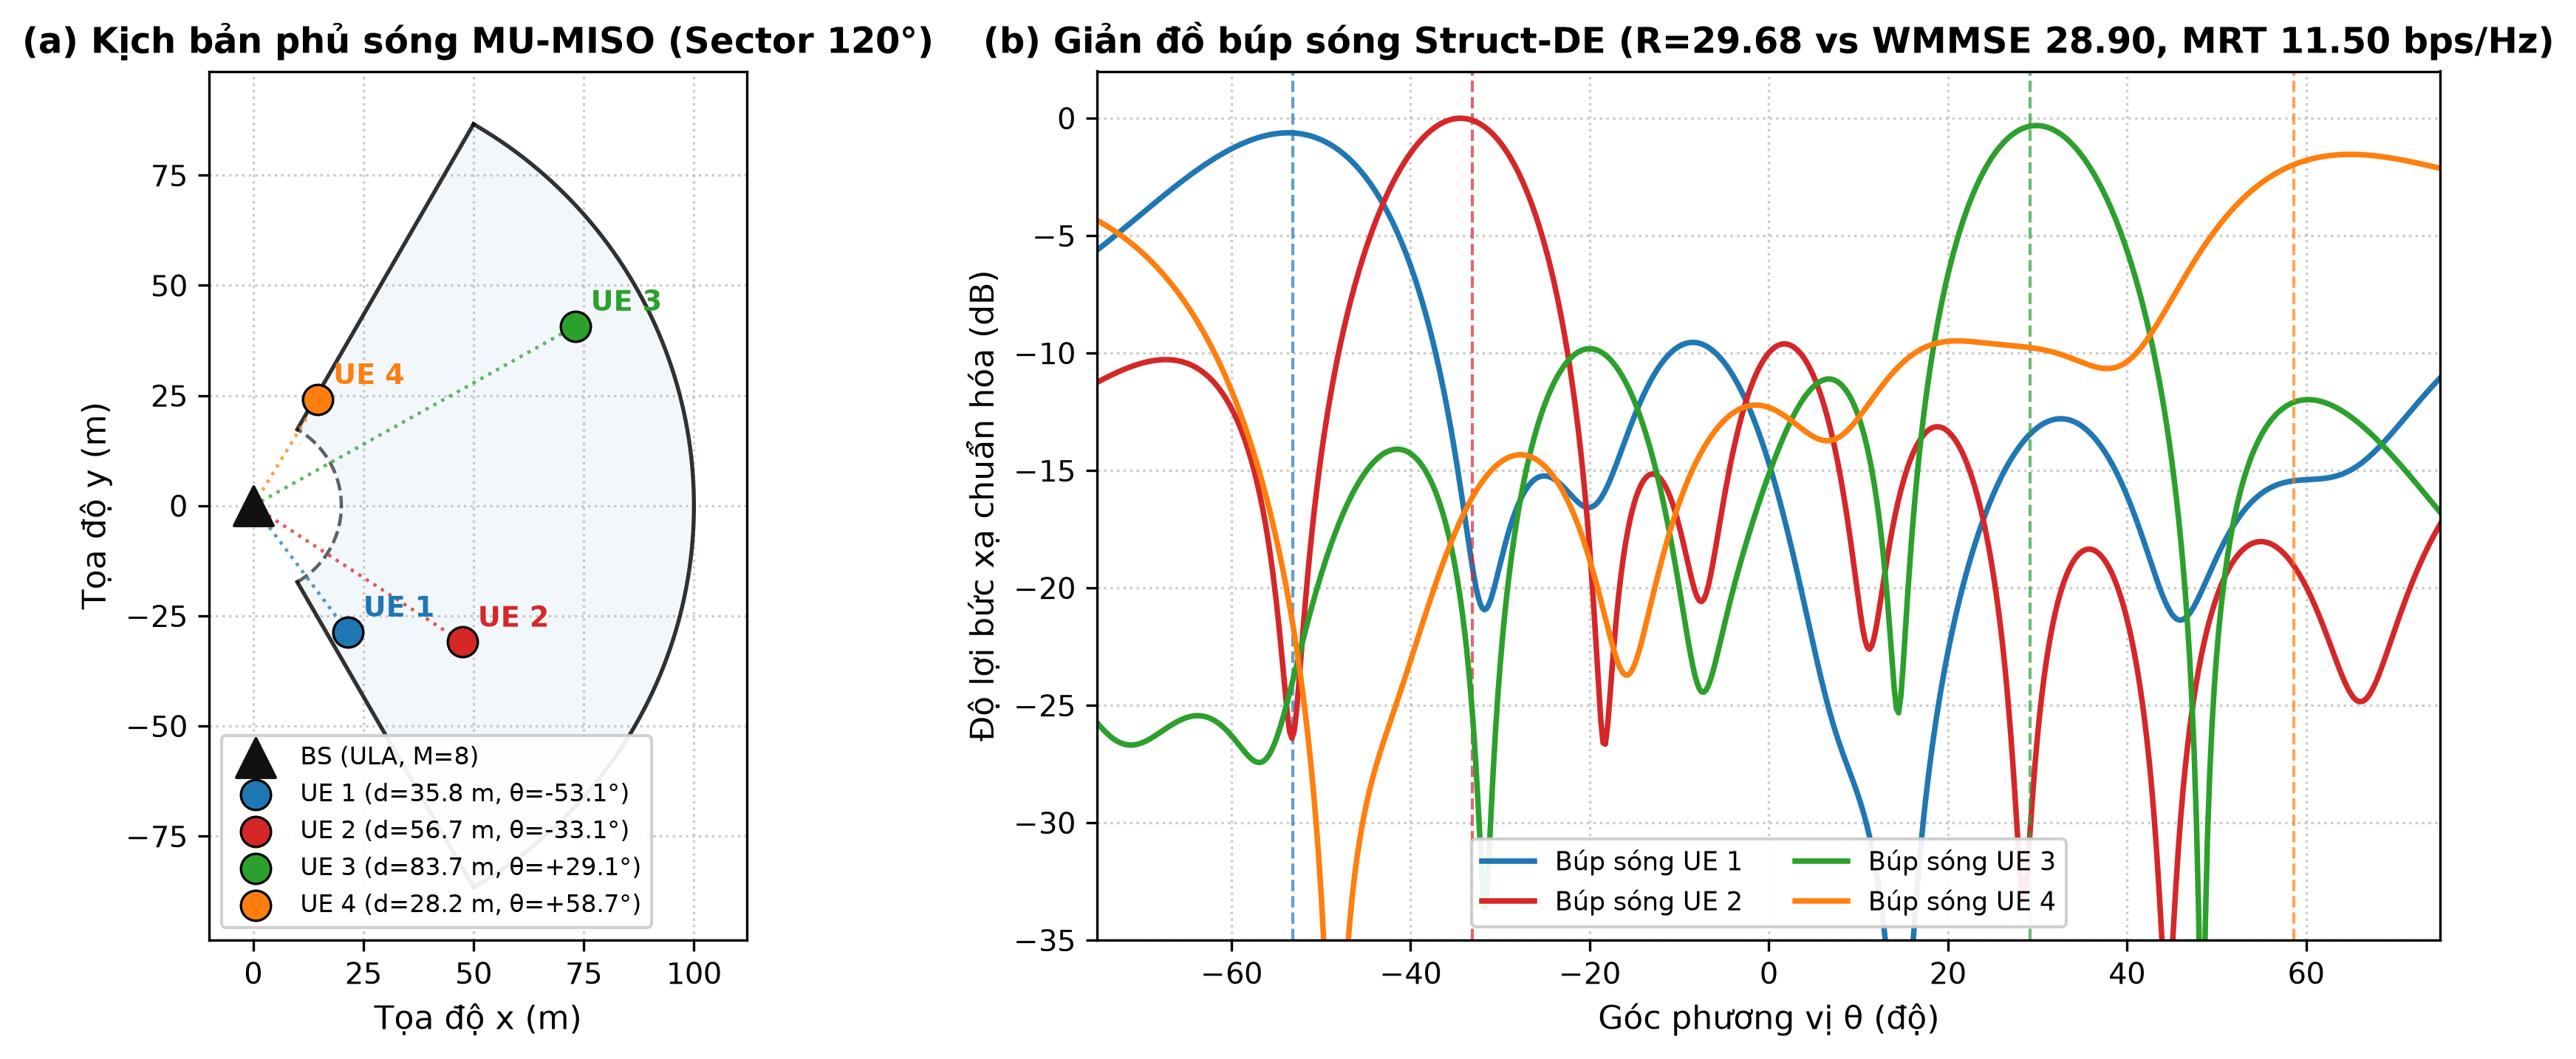
\includegraphics[width=0.98\linewidth]{../results/figures/fig1_geometry_beampattern.png}
    \caption{(a) Kịch bản phân bố người dùng trong sector $120^\circ$; (b) Giản đồ búp sóng chuẩn hóa của \texttt{Struct-DE} tại $M=8, K=4, P_{\max}=20$\,dBm.}
    \label{fig:geom}
\end{figure}

\begin{table}[H]
    \centering
    \caption{Tọa độ, khoảng cách, góc phương vị và suy hao đường truyền của 4 người dùng mẫu}
    \label{tab:ue}
    \begin{tabular}{l c c c c c}
        \toprule
        \textbf{Người dùng} & \textbf{$x$ (m)} & \textbf{$y$ (m)} & \textbf{$d_k$ (m)} & \textbf{$\theta_k$} & \textbf{PL (dB)} \\
        \midrule
        UE 1 & 21.48 & -28.65 & 35.81 & -53.14$^\circ$ & 89.94 \\
        UE 2 & 47.48 & -30.95 & 56.68 & -33.10$^\circ$ & 95.93 \\
        UE 3 & 73.09 & 40.76 & 83.69 & +29.14$^\circ$ & 101.00 \\
        UE 4 & 14.69 & 24.12 & 28.24 & +58.66$^\circ$ & 86.85 \\
        \bottomrule
    \end{tabular}
\end{table}

\subsection{Tổng tốc độ bit trung bình theo công suất phát $P_{\max}$}
Hình \ref{fig:power} và Bảng \ref{tab:power} trình bày tổng tốc độ bit trung bình trên 100 hiện thực kênh Rician khi công suất phát BS thay đổi từ $0$\,dBm đến $30$\,dBm ($M=8, K=4$).

\begin{figure}[H]
    \centering
    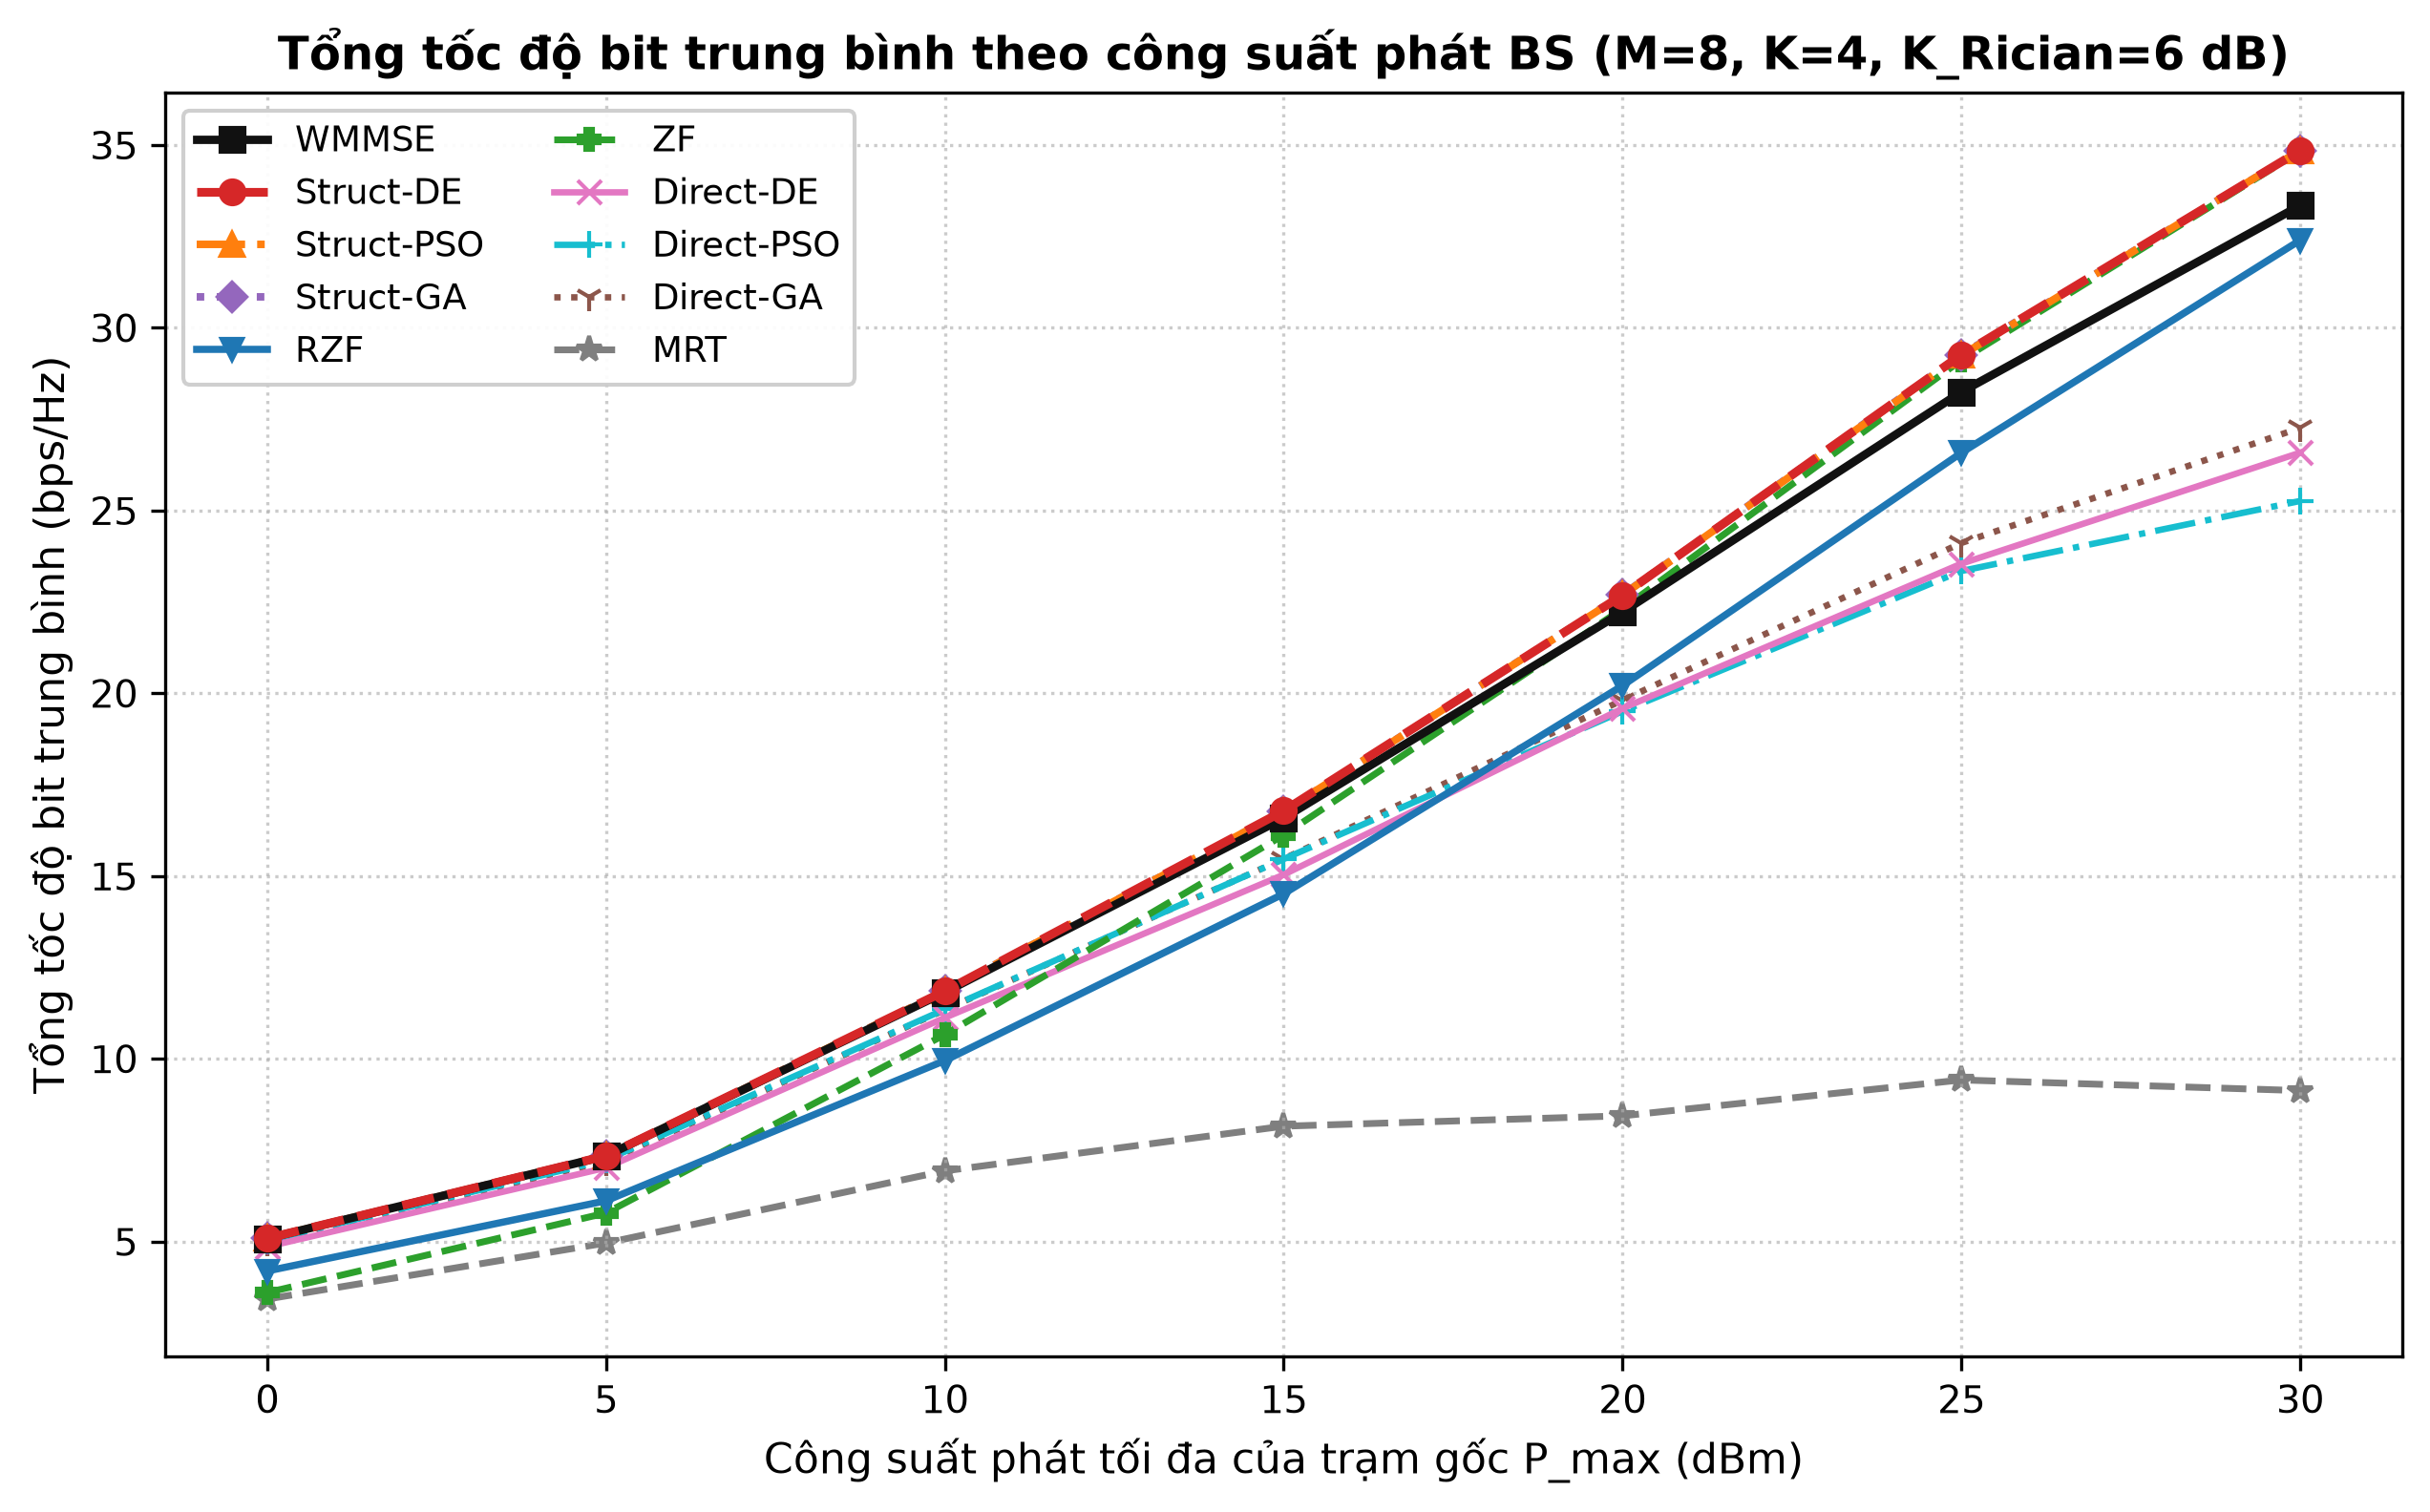
\includegraphics[width=0.88\linewidth]{../results/figures/fig2_sumrate_vs_power.png}
    \caption{Tổng tốc độ bit trung bình theo công suất phát trạm gốc $P_{\max}$ ($M=8, K=4, K_{\text{Rician}}=6$\,dB).}
    \label{fig:power}
\end{figure}

\begin{table}[H]
    \centering
    \caption{Tổng tốc độ bit trung bình (bps/Hz) theo công suất phát $P_{\max}$ ($M=8, K=4$)}
    \label{tab:power}
    \begin{tabular}{c c c c c c c c}
        \toprule
        \textbf{$P_{\max}$ (dBm)} & \textbf{MRT} & \textbf{ZF} & \textbf{RZF} & \textbf{WMMSE} & \textbf{Direct-DE} & \textbf{Struct-DE} & \textbf{Struct-PSO} \\
        \midrule
        0 & 3.42 & 3.60 & 4.19 & 5.08 & 4.86 & \textbf{5.08} & 5.09 \\
        5 & 4.96 & 5.78 & 6.11 & 7.34 & 7.02 & \textbf{7.34} & 7.34 \\
        10 & 6.93 & 10.66 & 9.95 & 11.82 & 11.12 & \textbf{11.85} & 11.85 \\
        15 & 8.15 & 16.12 & 14.51 & 16.59 & 15.04 & \textbf{16.78} & 16.77 \\
        20 & 8.44 & 22.31 & 20.21 & 22.22 & 19.59 & \textbf{22.68} & 22.69 \\
        25 & 9.42 & 29.12 & 26.58 & 28.25 & 23.55 & \textbf{29.26} & 29.25 \\
        30 & 9.13 & 34.83 & 32.40 & 33.35 & 26.58 & \textbf{34.85} & 34.85 \\
        \bottomrule
    \end{tabular}
\end{table}

\textbf{Phân tích định lượng:}
\begin{itemize}
    \item \emph{Miền công suất thấp ($0\text{--}5$\,dBm):} \texttt{RZF} (4.19\,bps/Hz tại $0$\,dBm) vượt cả \texttt{MRT} (3.42) và \texttt{ZF} (3.60) nhờ cân bằng giữa độ lợi mảng và triệt nhiễu. Đặc biệt, \texttt{Struct-DE/PSO/GA} đạt 5.08\,bps/Hz (ngang bằng và nhỉnh hơn nhẹ \texttt{WMMSE} 5.08\,bps/Hz), thậm chí các giải thuật trực tiếp (\texttt{Direct-DE/PSO/GA}) đạt $4.86\text{--}5.02$\,bps/Hz cũng vượt xa \texttt{MRT}, \texttt{ZF} và \texttt{RZF} nhờ biết dồn công suất vào các người dùng gần có kênh mạnh.
    \item \emph{Miền công suất cao ($20\text{--}30$\,dBm):} \texttt{MRT} nhanh chóng bão hòa quanh 9.13\,bps/Hz do nhiễu đồng kênh MUI tăng cùng tỷ lệ với tín hiệu mong muốn. Ngược lại, \texttt{Struct-DE/PSO/GA} tăng gần tuyến tính theo $P_{\max}$ (dBm), đạt 34.85\,bps/Hz tại $30$\,dBm (cải thiện +281.8\% so với MRT và cao hơn \texttt{WMMSE} bị cắt cụt ở 100 vòng lặp là 33.35\,bps/Hz do WMMSE hội tụ chậm khi suy hao gần--xa chênh lệch mạnh). Lưu ý \texttt{RZF} chuẩn hóa toàn ma trận đạt 32.40\,bps/Hz thấp hơn \texttt{ZF} (34.83\,bps/Hz) ở $30$\,dBm vì nghịch đảo kênh không chuẩn hóa cột phân bổ quá nhiều công suất cho người dùng ở xa \cite{peel2005}.
\end{itemize}

\subsection{Khảo sát ảnh hưởng của số lượng anten trạm gốc $M$}
Hình \ref{fig:ant} và Bảng \ref{tab:ant} đánh giá hiệu năng khi tăng $M \in \{4, 8, 12, 16, 24, 32\}$ tại $K=4, P_{\max}=20$\,dBm.

\begin{figure}[H]
    \centering
    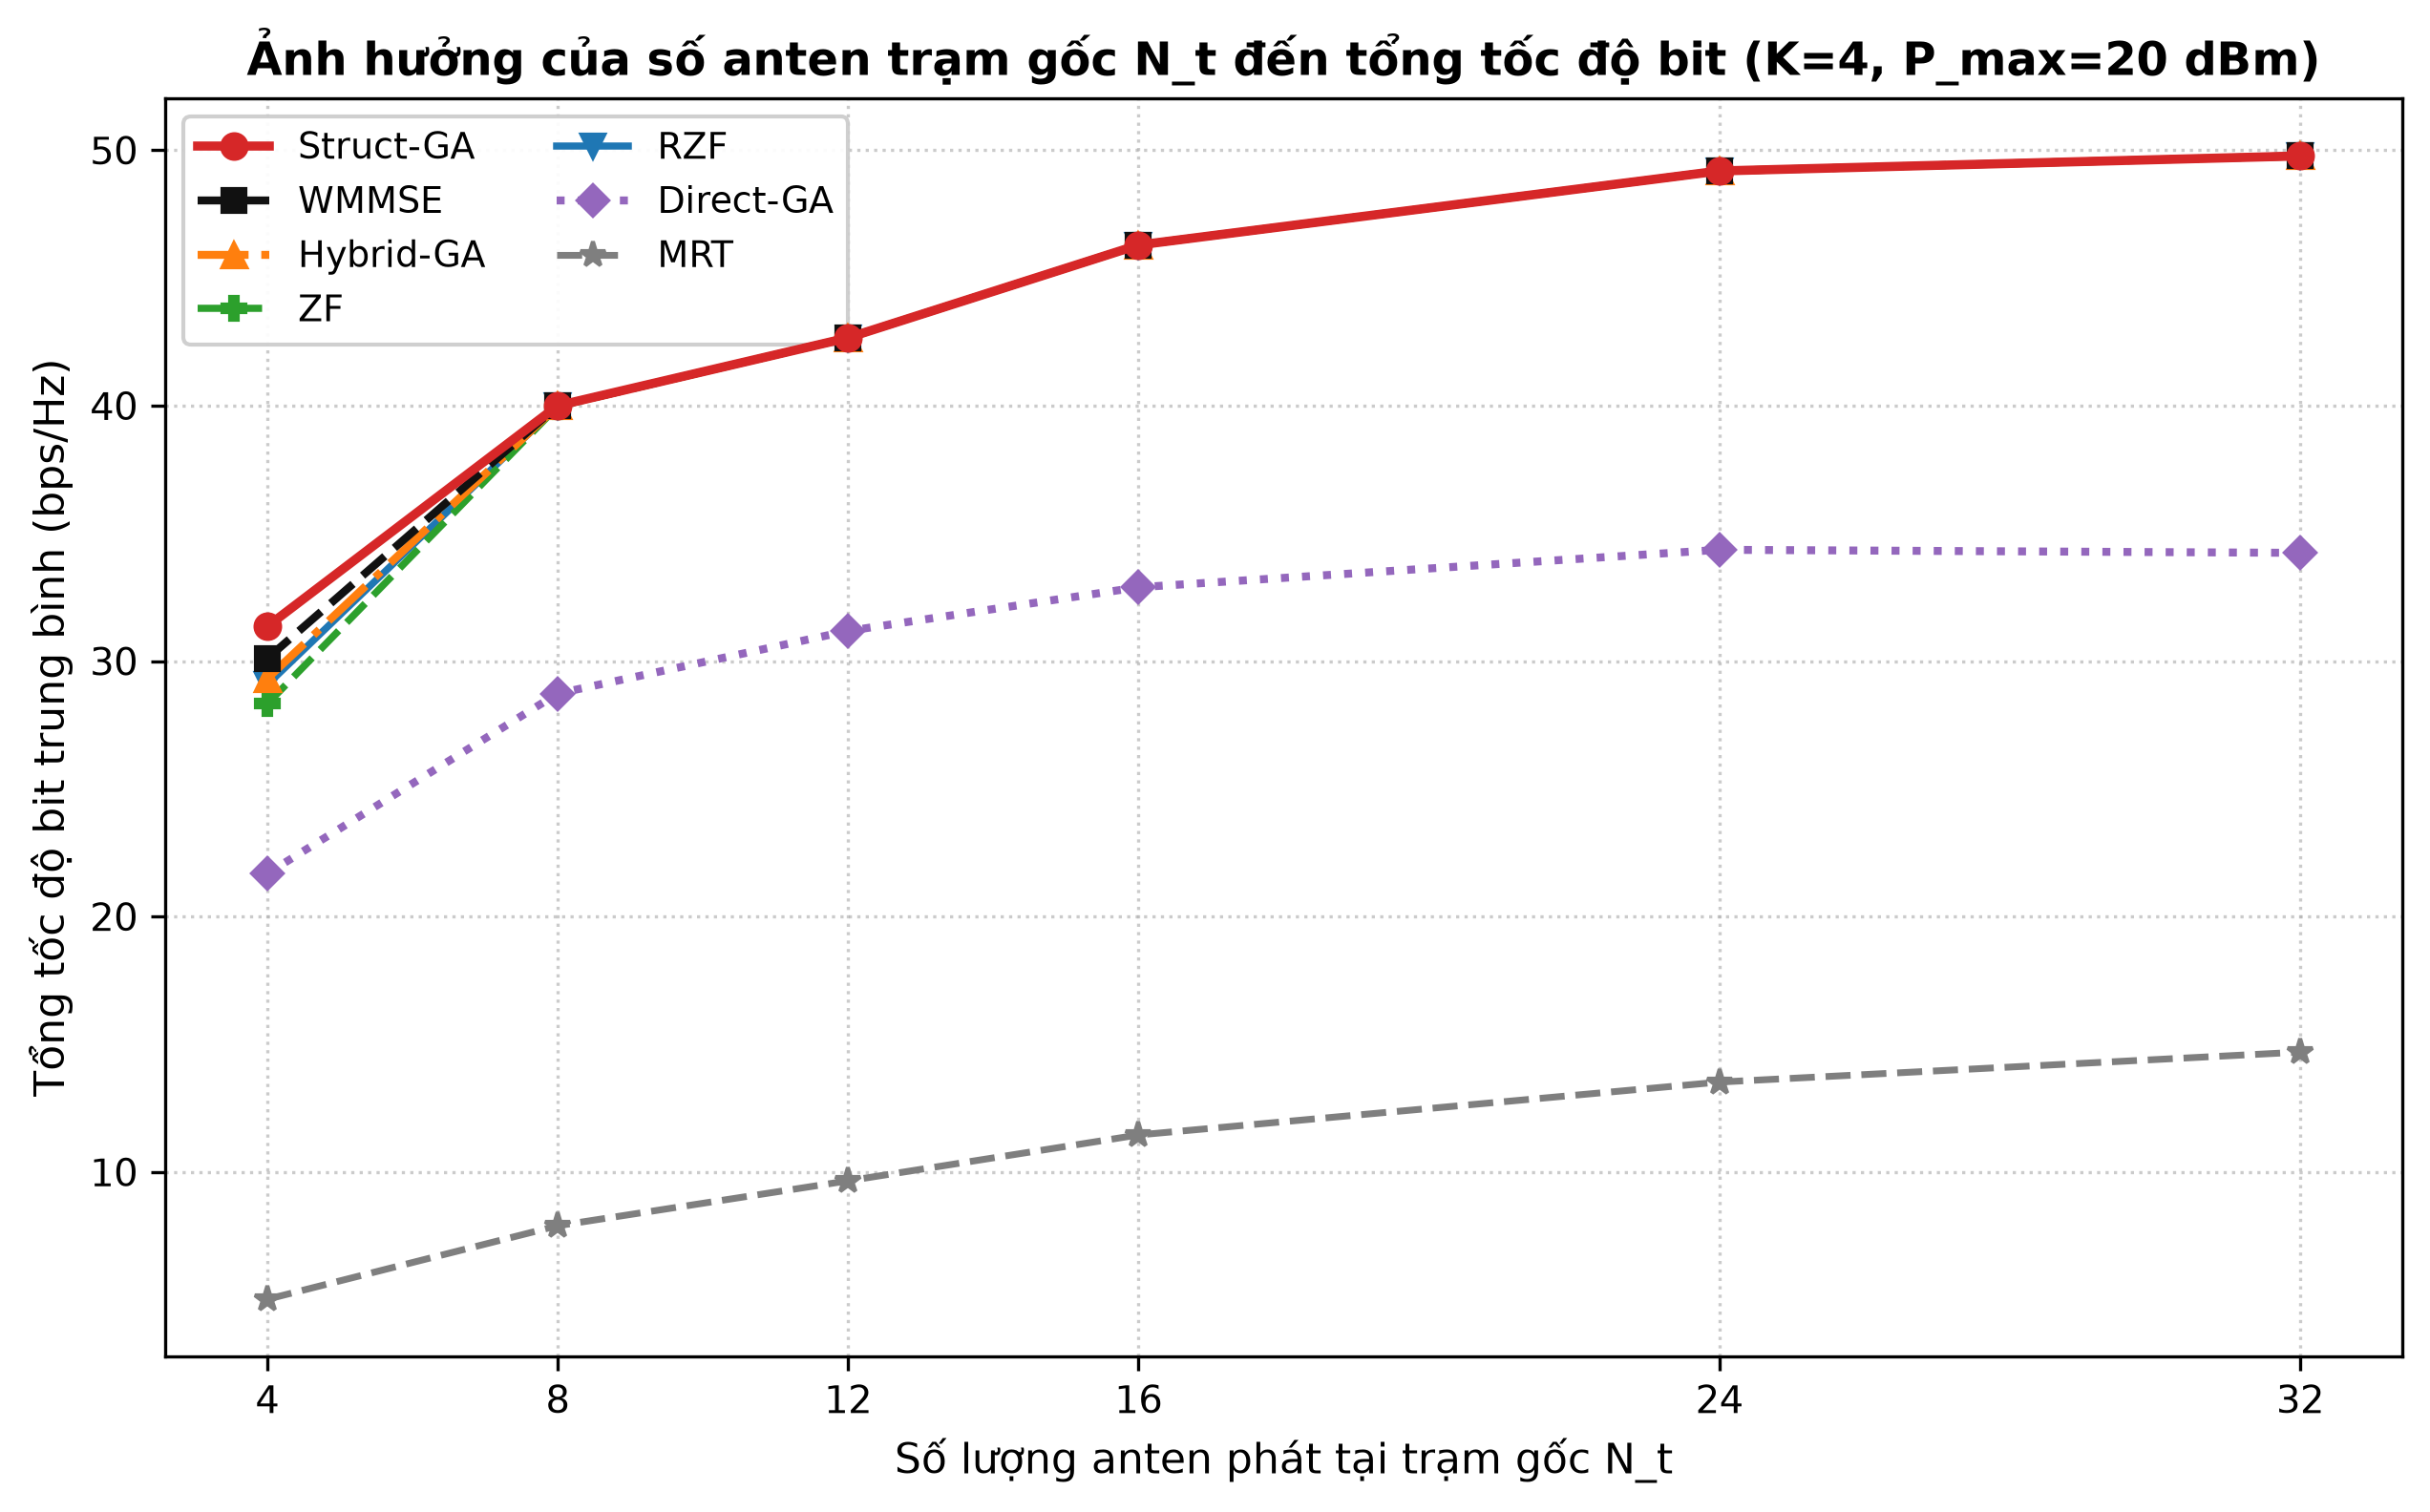
\includegraphics[width=0.88\linewidth]{../results/figures/fig3_sumrate_vs_antennas.png}
    \caption{Ảnh hưởng của số lượng anten BS $M$ đến tổng tốc độ bit trung bình ($K=4, P_{\max}=20$\,dBm).}
    \label{fig:ant}
\end{figure}

\begin{table}[H]
    \centering
    \caption{Tổng tốc độ bit trung bình (bps/Hz) và thời gian chạy \texttt{Struct-DE} theo số anten $M$ ($K=4, P_{\max}=20$\,dBm)}
    \label{tab:ant}
    \begin{tabular}{c c c c c c c c c}
        \toprule
        \textbf{$M$} & \textbf{$2MK$} & \textbf{MRT} & \textbf{ZF} & \textbf{RZF} & \textbf{WMMSE} & \textbf{Direct-DE} & \textbf{Struct-DE} & \textbf{Time (ms)} \\
        \midrule
        4 & 32 & 5.43 & 12.33 & 12.47 & 16.33 & 15.00 & \textbf{16.64} & 16.20 \\
        8 & 64 & 8.99 & 21.85 & 19.78 & 21.84 & 19.52 & \textbf{22.28} & 16.04 \\
        12 & 96 & 11.36 & 25.87 & 23.57 & 25.27 & 21.44 & \textbf{25.92} & 15.98 \\
        16 & 128 & 12.91 & 28.51 & 26.04 & 27.61 & 22.90 & \textbf{28.54} & 16.00 \\
        24 & 192 & 16.30 & 31.28 & 29.40 & 30.39 & 24.09 & \textbf{31.29} & 15.65 \\
        32 & 256 & 17.21 & 32.92 & 30.63 & 31.60 & 24.53 & \textbf{32.93} & 15.57 \\
        \bottomrule
    \end{tabular}
\end{table}

\textbf{Nhận xét quan trọng về giới hạn số chiều:} Khi $M=K=4$ (không có bậc tự do không gian dư), \texttt{ZF} bị khuếch đại tạp âm nghiêm trọng (12.33\,bps/Hz), trong khi ngay cả \texttt{Direct-DE} (32 biến) đã đạt 15.00\,bps/Hz và \texttt{Struct-DE} đạt 16.64\,bps/Hz. Tuy nhiên, khi tăng $M$ từ $4 \to 32$, tổng tốc độ bit của \texttt{Struct-DE} tăng mạnh +98.0\% (lên 32.93\,bps/Hz) với thời gian tính toán giữ gần như \textbf{hằng số} ($\approx 15.6\text{--}16.2$\,ms, chứng thực độ phức tạp $\mathcal{O}(K^3)$ độc lập với $M$). Trái lại, \texttt{Direct-DE} gặp \emph{lời nguyền số chiều} khi số biến phình lên $2MK = 256$: hiệu năng chững lại ở 24.53\,bps/Hz (kém \texttt{Struct-DE} tới 8.40\,bps/Hz) đồng thời thời gian chạy tăng gần gấp đôi.

\subsection{Khảo sát ảnh hưởng của số người dùng $K$ và chế độ quá tải ($K > M$)}
Hình \ref{fig:users} và Bảng \ref{tab:users} khảo sát khi số người dùng tăng $K \in \{2, 4, 6, 8, 10\}$ với $M=8$ cố định.

\begin{figure}[H]
    \centering
    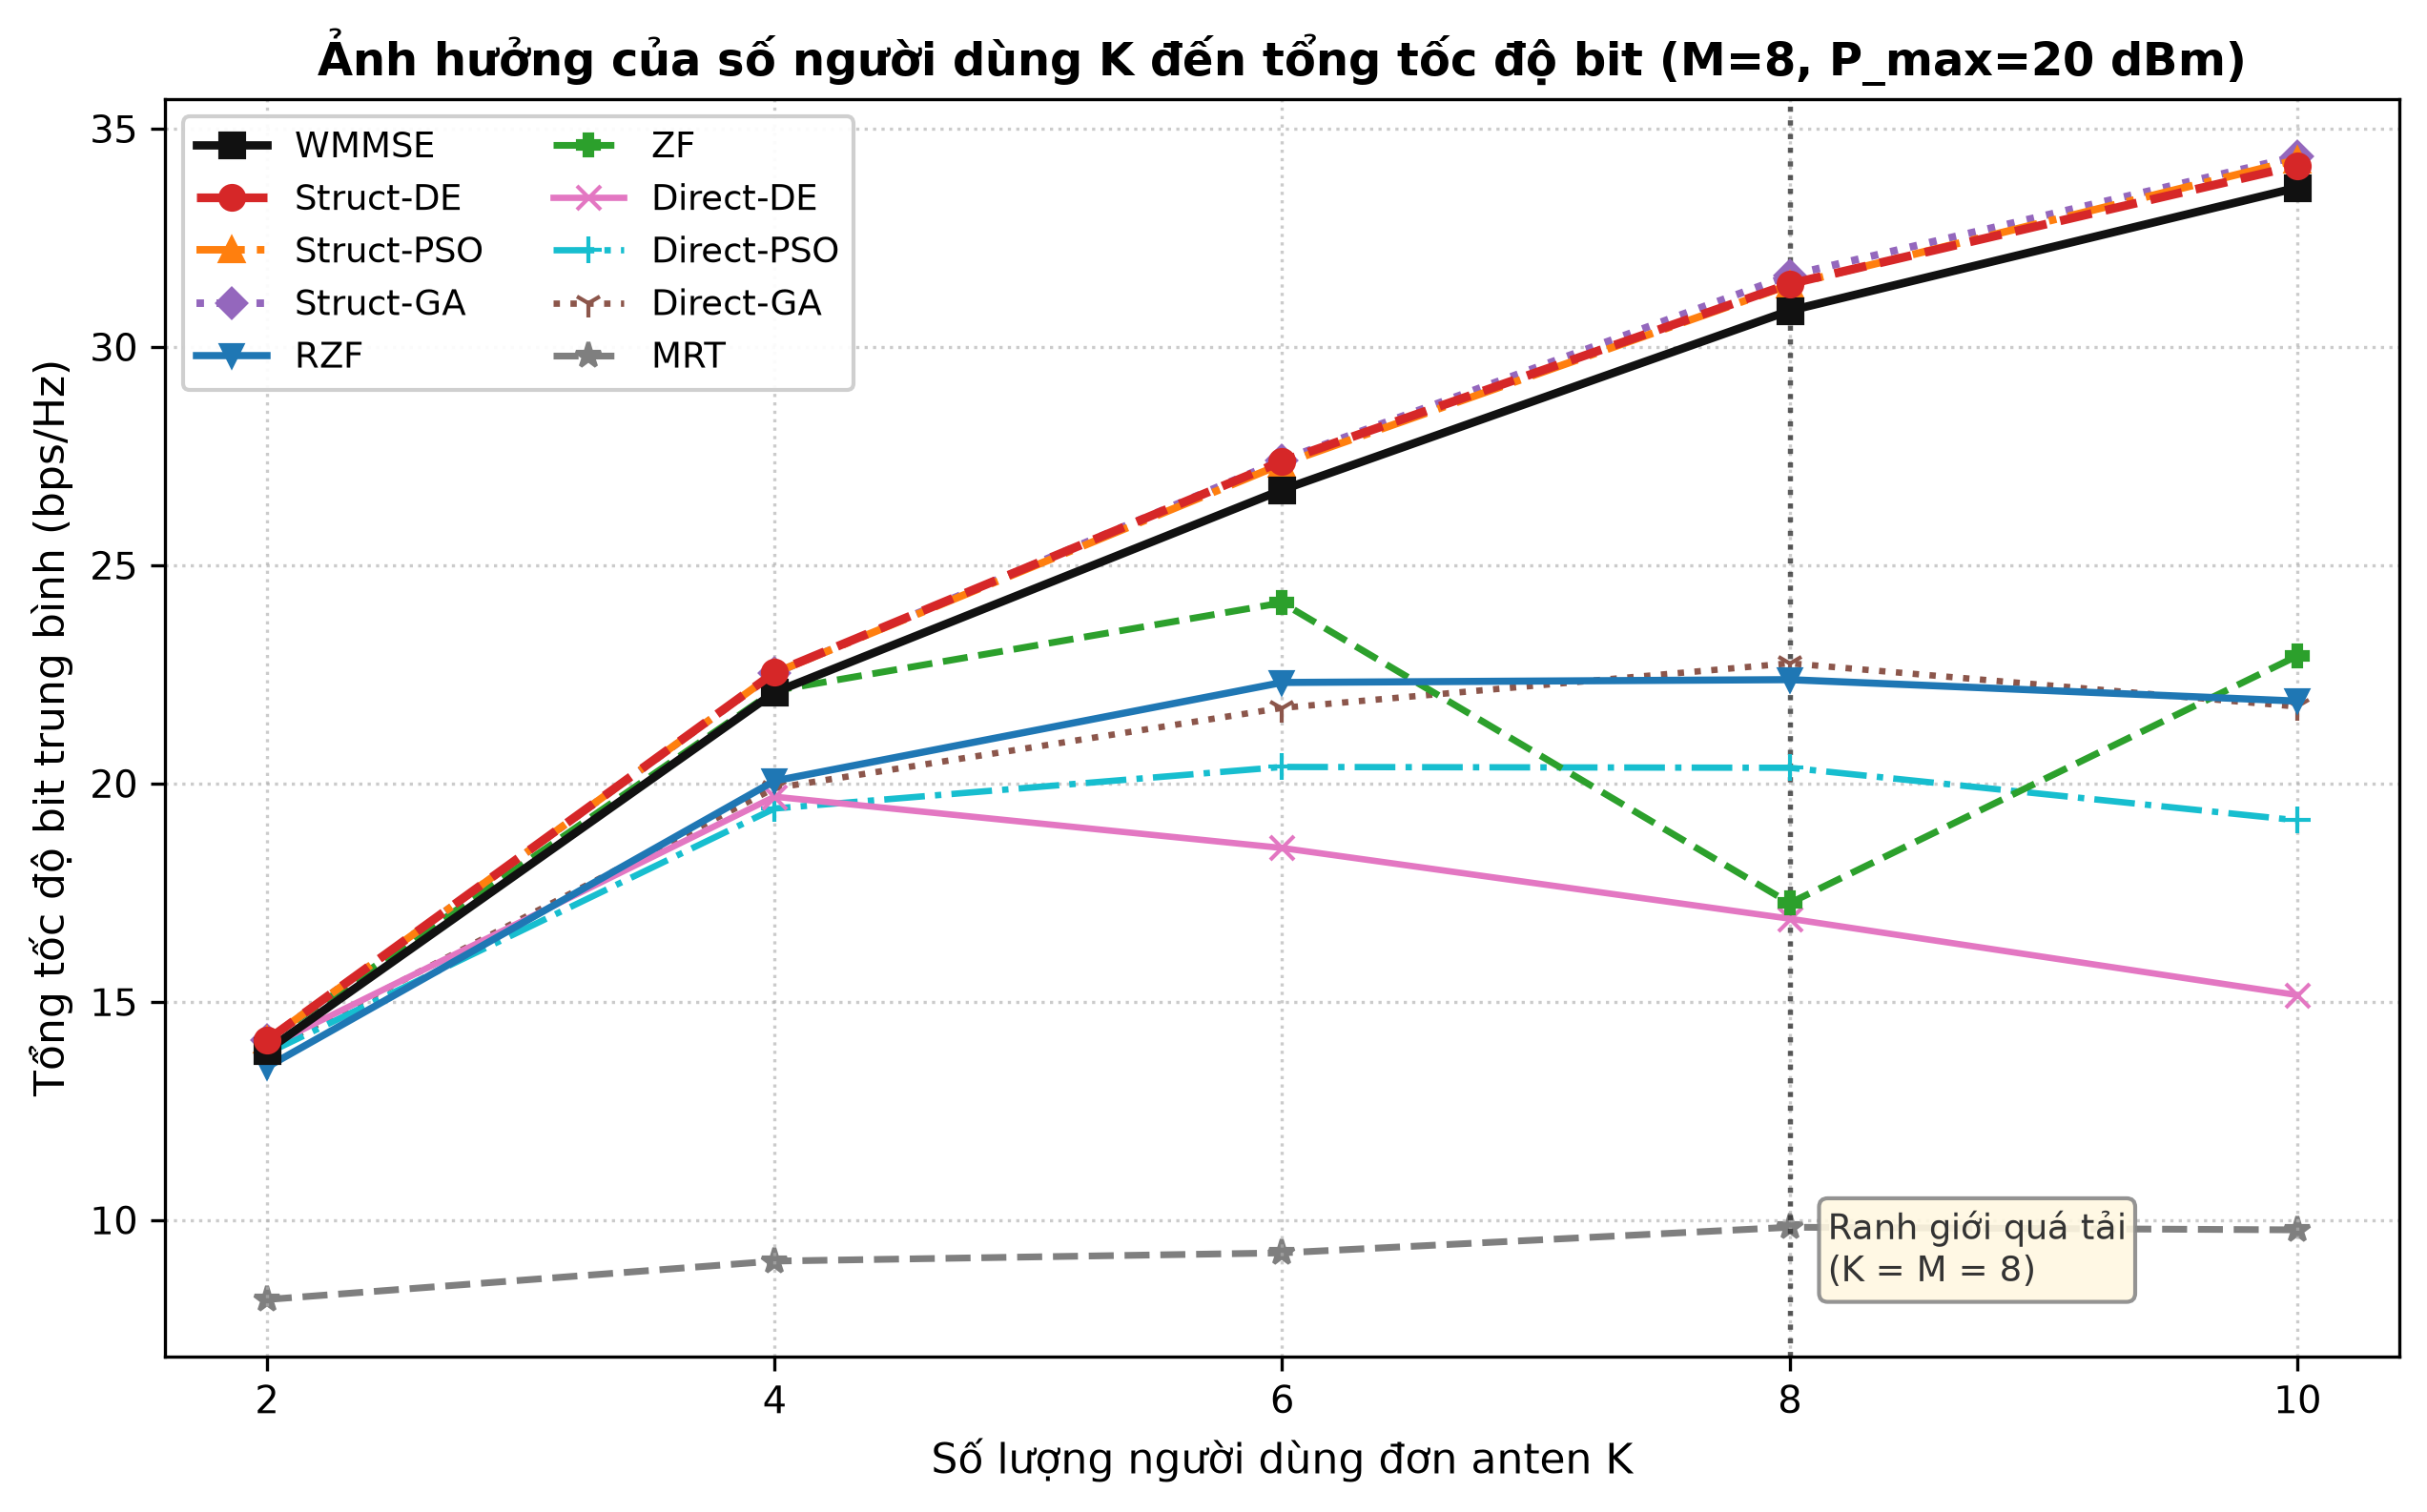
\includegraphics[width=0.88\linewidth]{../results/figures/fig4_sumrate_vs_users.png}
    \caption{Ảnh hưởng của số người dùng $K$ đến tổng tốc độ bit trung bình ($M=8, P_{\max}=20$\,dBm), bao gồm vùng quá tải $K > M$.}
    \label{fig:users}
\end{figure}

\begin{table}[H]
    \centering
    \caption{Tổng tốc độ bit trung bình (bps/Hz) theo số người dùng $K$ ($M=8, P_{\max}=20$\,dBm)}
    \label{tab:users}
    \begin{tabular}{c c c c c c c c}
        \toprule
        \textbf{$K$} & \textbf{MRT} & \textbf{ZF} & \textbf{RZF} & \textbf{WMMSE} & \textbf{Direct-DE} & \textbf{Struct-DE} & \textbf{Struct-PSO} \\
        \midrule
        2 & 8.18 & 14.11 & 13.50 & 13.88 & 13.96 & \textbf{14.12} & 14.12 \\
        4 & 9.06 & 22.12 & 20.06 & 22.09 & 19.70 & \textbf{22.54} & 22.53 \\
        6 & 9.24 & 24.14 & 22.31 & 26.72 & 18.52 & \textbf{27.38} & 27.32 \\
        8 & 9.83 & 17.26 & 22.38 & 30.83 & 16.90 & \textbf{31.44} & 31.42 \\
        10 & 9.77 & 22.92 & 21.89 & 33.65 & 15.15 & \textbf{34.15} & 34.29 \\
        \bottomrule
    \end{tabular}
\end{table}

Khi $K$ tăng từ $2 \to 8$, \texttt{Struct-DE} khai thác độ lợi ghép kênh không gian và đa dạng đa người dùng để tăng tổng tốc độ từ 14.12 lên 31.44\,bps/Hz, và tiếp tục đạt 34.15\,bps/Hz ngay cả trong vùng quá tải $K=10 > M=8$. Ngược lại, \texttt{ZF} đạt đỉnh tại $K=6$ rồi \textbf{sụt giảm mạnh tại ranh giới vuông $K=M=8$} (chỉ còn 17.26\,bps/Hz) do hiện tượng suy giảm giá trị kỳ dị nhỏ nhất khiến nghịch đảo kênh khuếch đại tạp âm cực mạnh; sang $K=10$, giả nghịch đảo Moore--Penrose không còn ép triệt nhiễu tuyệt đối nên hồi phục nhẹ lên 22.92\,bps/Hz nhưng vẫn kém \texttt{Struct-DE} hơn $11.2$\,bps/Hz. Với \texttt{Direct-DE} (số biến $2MK$ tăng từ $32 \to 160$), hiệu năng bắt đầu suy giảm ngay từ $K \ge 6$ xuống còn 15.15\,bps/Hz. Trong khi đó, nhờ cơ chế cắt ngưỡng công suất không âm $p_k = \max(z_k, 0)$, \texttt{Struct-DE/PSO/GA} tự động thực hiện lập lịch người dùng ngầm (tắt các UE yếu/nhiễu nặng) và vượt cả \texttt{WMMSE} (33.65\,bps/Hz).

\subsection{Khảo sát bổ sung theo hệ số Rician $K$-factor}
\begin{figure}[H]
    \centering
    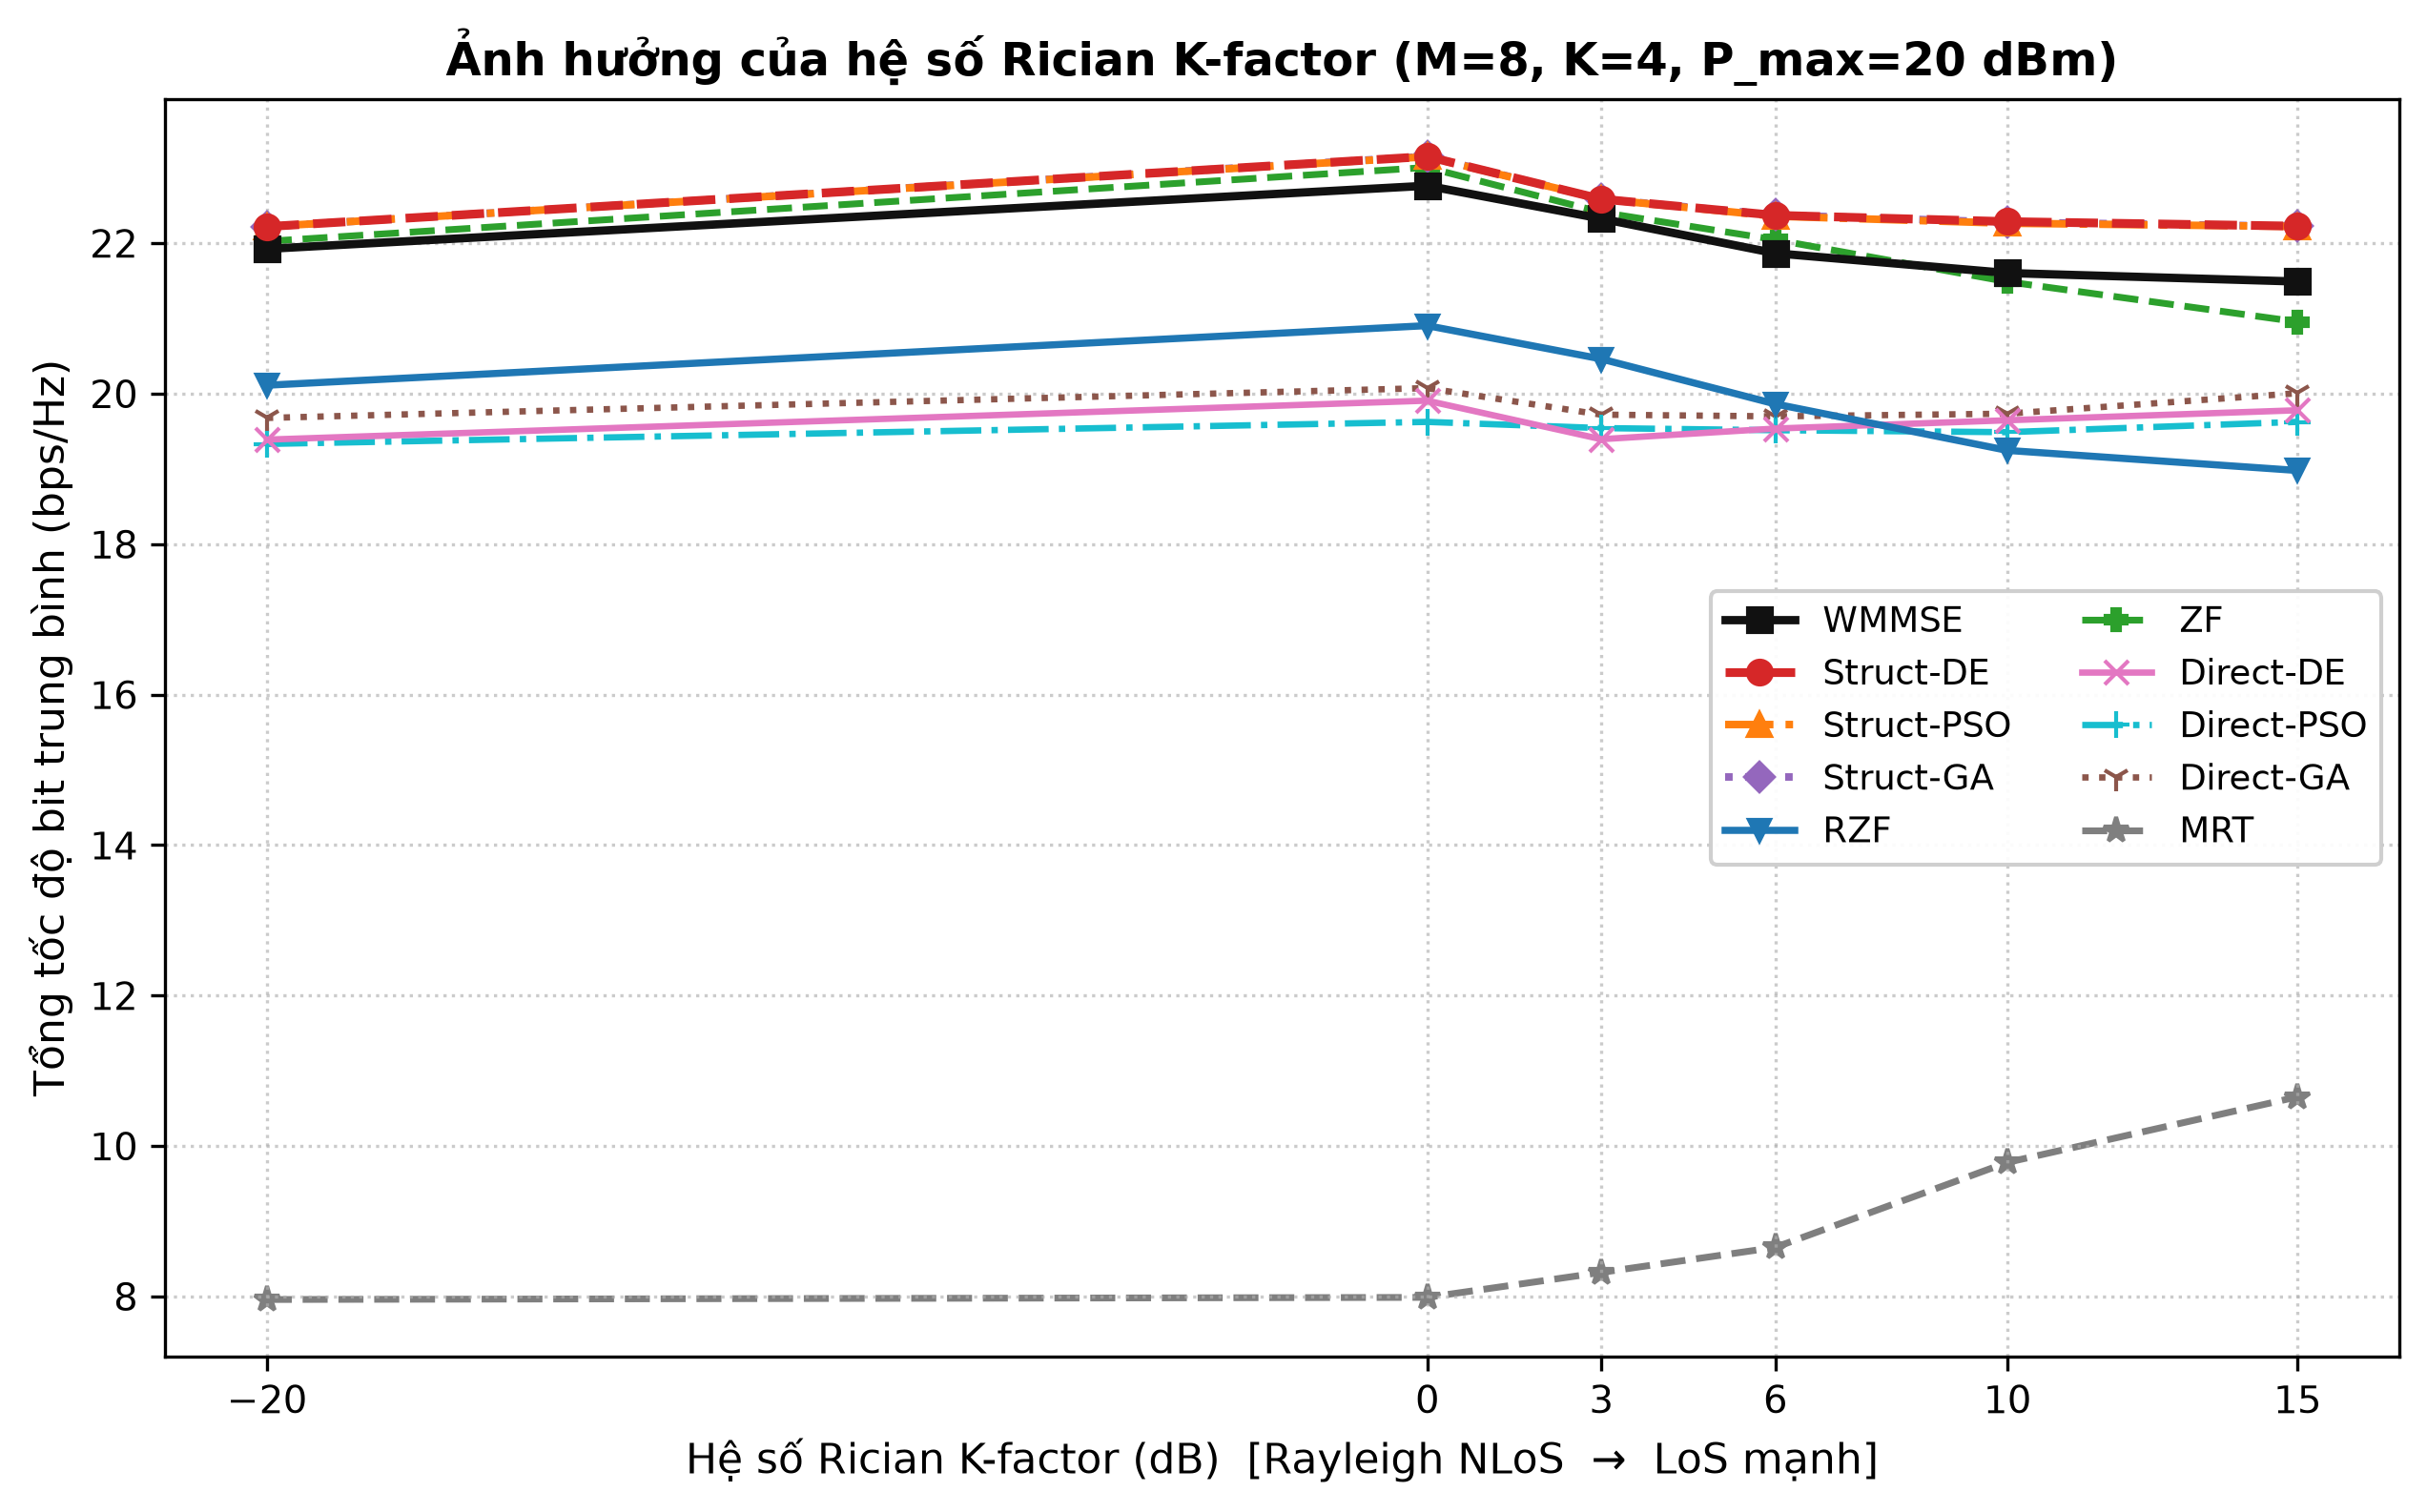
\includegraphics[width=0.88\linewidth]{../results/figures/fig5_sumrate_vs_rician_k.png}
    \caption{Ảnh hưởng của hệ số Rician $K$-factor từ tán xạ Rayleigh ($-20$\,dB) tới LoS mạnh ($15$\,dB) tại $M=8, K=4, P_{\max}=20$\,dBm.}
    \label{fig:rician}
\end{figure}
Khi $K_{\text{Rician}}$ tăng từ $-20$\,dB (Rayleigh NLoS) lên $+15$\,dB (LoS mạnh), độ tương quan không gian giữa các người dùng ở góc gần nhau tăng khiến \texttt{ZF} (đạt đỉnh tại $0$\,dB) giảm xuống còn 20.96\,bps/Hz và \texttt{RZF} giảm còn 18.98\,bps/Hz; ngược lại \texttt{MRT} cải thiện từ 7.96 lên 10.65\,bps/Hz nhờ búp sóng LoS ULA ổn định hơn pha-đinh Rayleigh sâu. Trong suốt dải khảo sát, \texttt{Struct-DE} duy trì hiệu năng cao nhất và rất ổn định (22.22 $\to$ 22.23\,bps/Hz).

\subsection{Phân tích sự hội tụ, độ ổn định và chi phí tính toán}
Hình \ref{fig:conv}, Hình \ref{fig:stab} và Bảng \ref{tab:stab} tổng hợp đường cong hội tụ trung bình $\pm 1\sigma$, phân bố độ ổn định trên 30 lần chạy độc lập và thời gian thực thi mỗi kênh tại cấu hình chuẩn ($M=8, K=4, P_{\max}=20$\,dBm).

\begin{figure}[H]
    \centering
    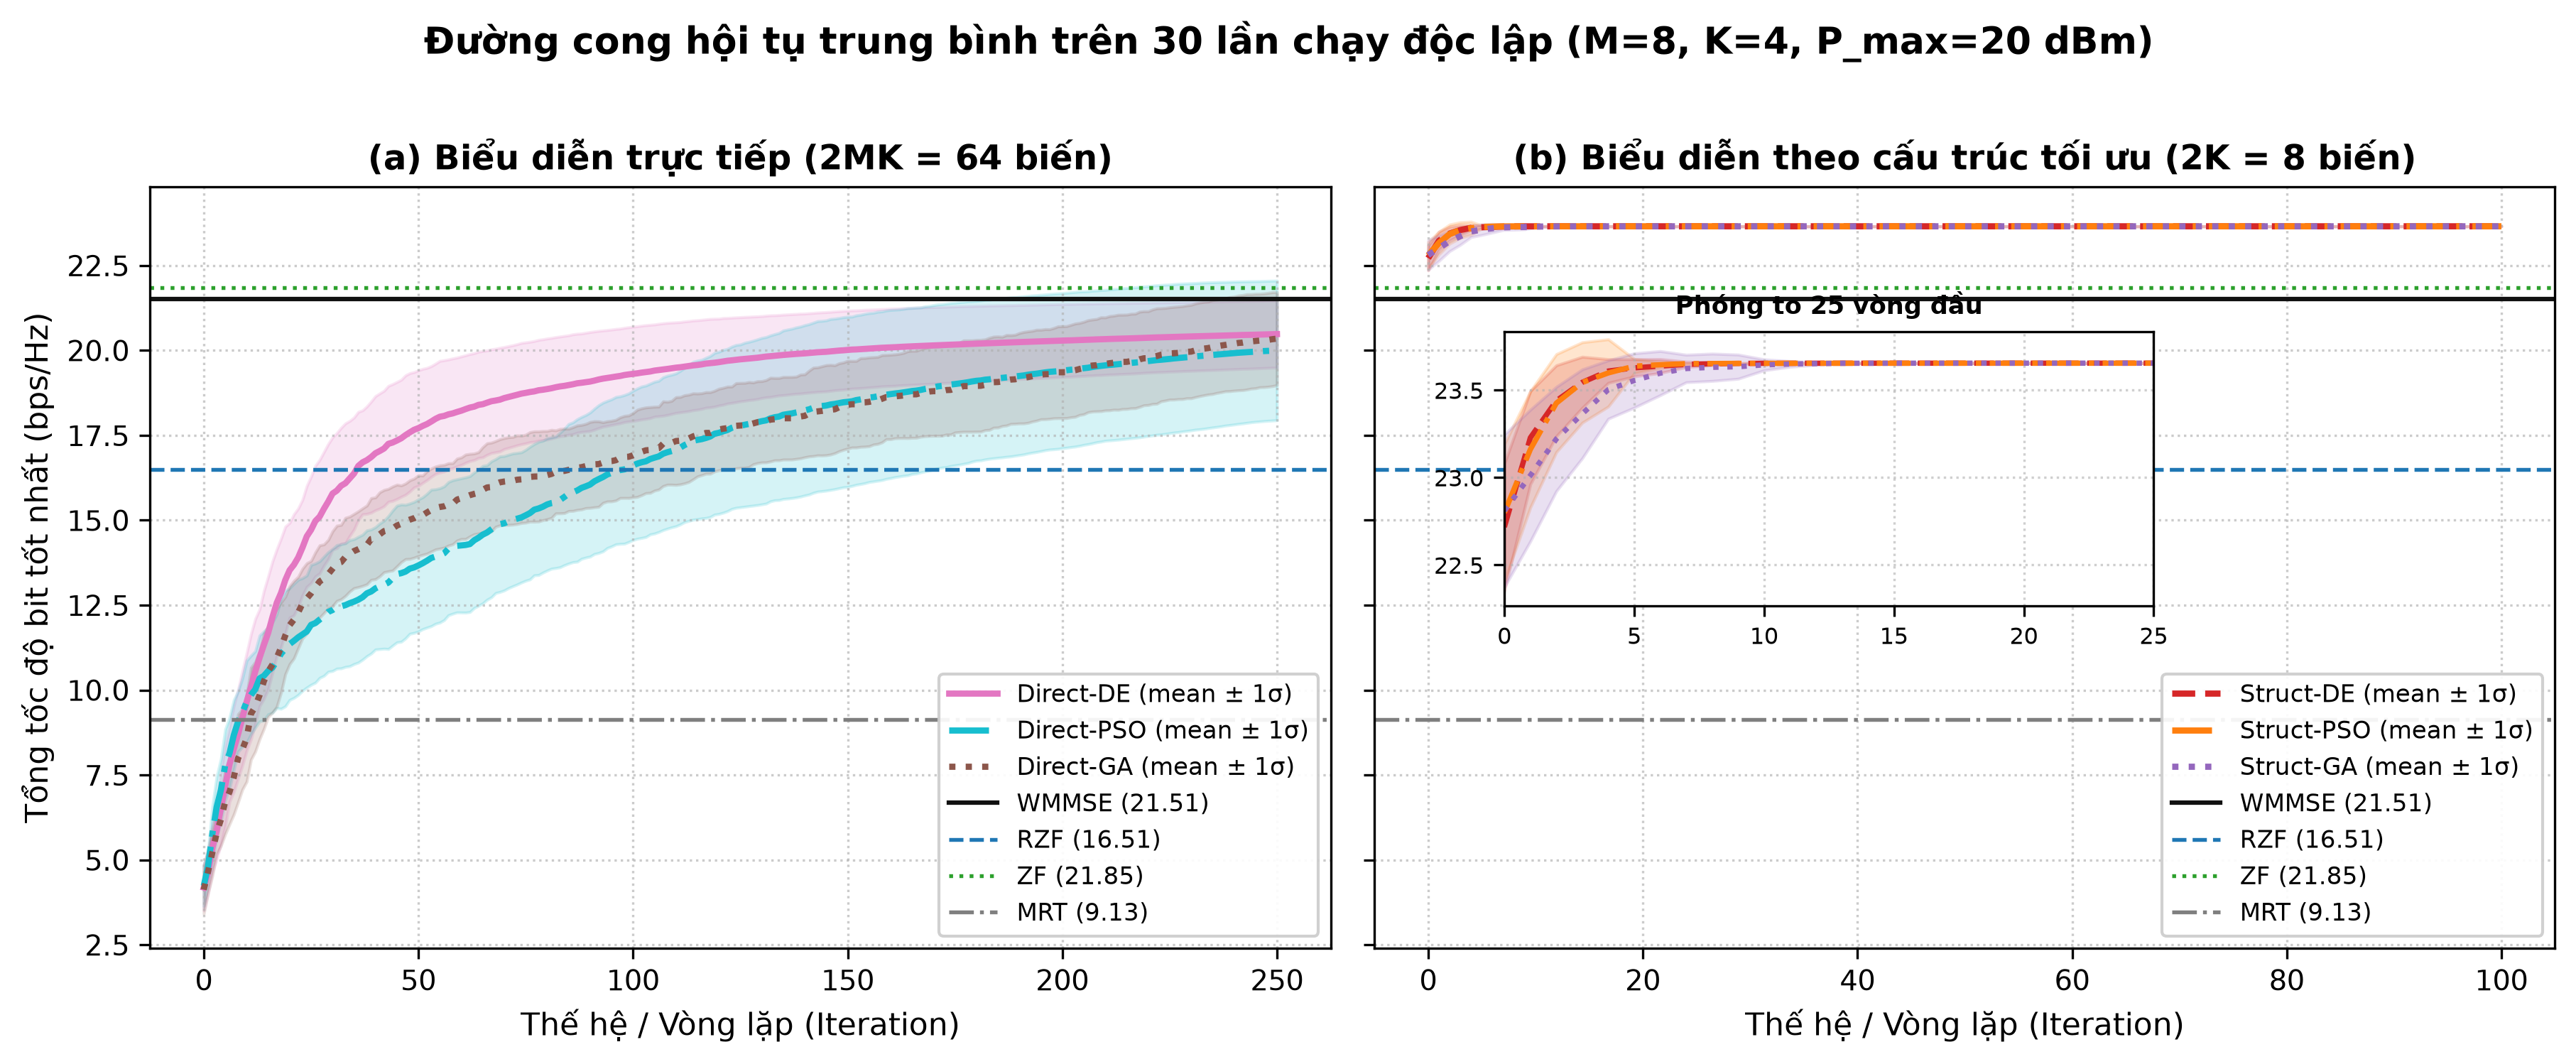
\includegraphics[width=0.98\linewidth]{../results/figures/fig6_convergence_curves.png}
    \caption{Đường cong hội tụ trung bình $\pm 1\sigma$ trên 30 lần chạy độc lập của (a) mã hóa trực tiếp $2MK=64$ biến và (b) mã hóa cấu trúc $2K=8$ biến.}
    \label{fig:conv}
\end{figure}

\begin{figure}[H]
    \centering
    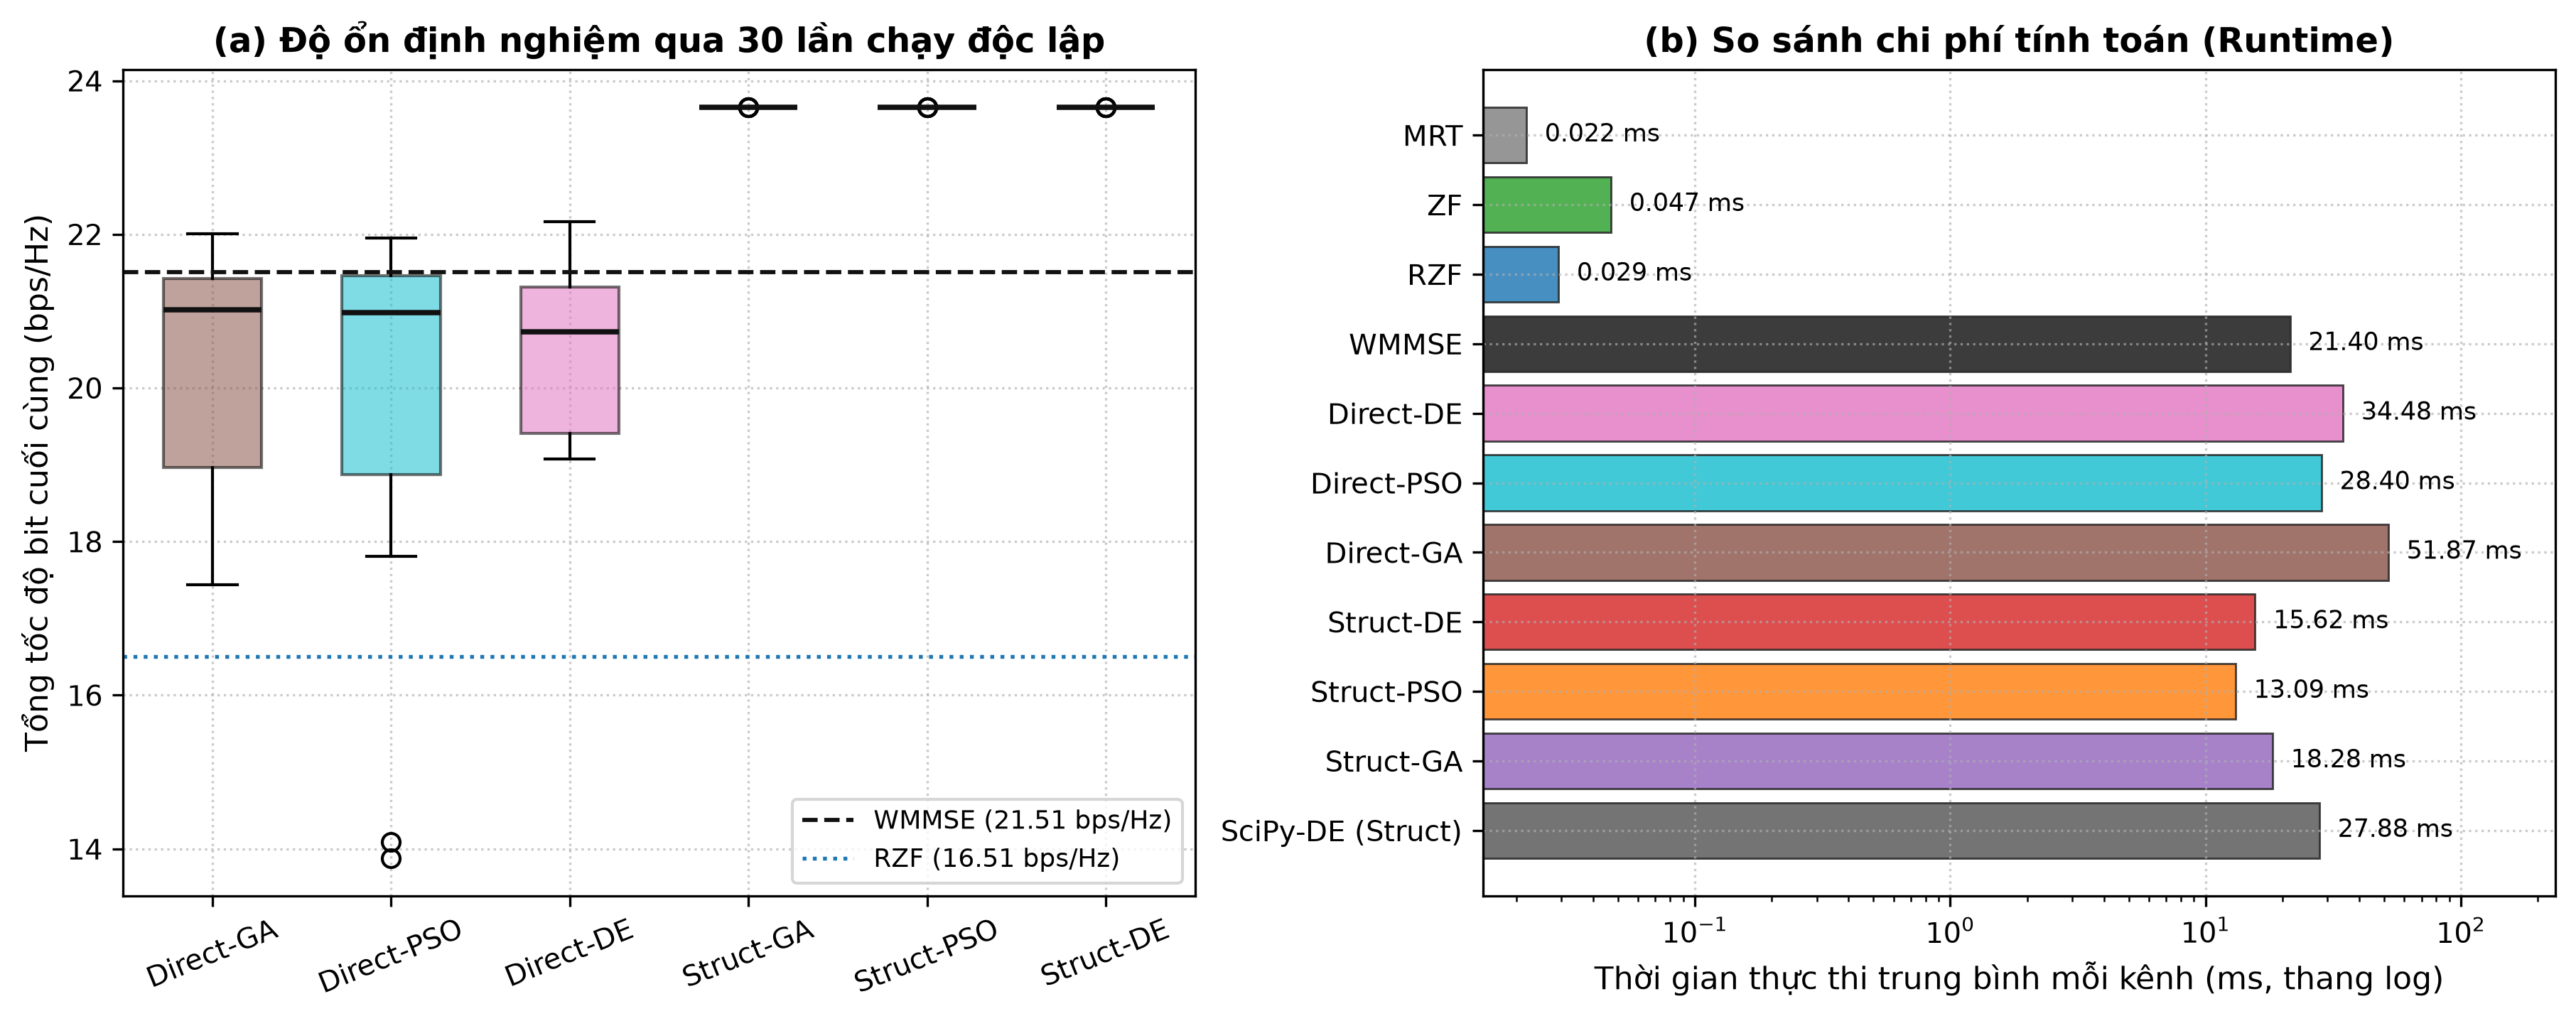
\includegraphics[width=0.98\linewidth]{../results/figures/fig7_stability_runtime.png}
    \caption{(a) Biểu đồ hộp đánh giá độ ổn định nghiệm cuối trên 30 lần chạy; (b) Thời gian tính toán trung bình mỗi kênh (thang log).}
    \label{fig:stab}
\end{figure}

\begin{table}[H]
    \centering
    \caption{Độ chính xác, độ ổn định (30 lần chạy) và chi phí tính toán tại $M=8, K=4, P_{\max}=20$\,dBm}
    \label{tab:stab}
    \begin{tabular}{l c c c c c c}
        \toprule
        \textbf{Phương pháp} & \textbf{Chiều} & \textbf{Mean (bps/Hz)} & \textbf{Std} & \textbf{CV} & \textbf{Runtime (ms)} & \textbf{Evals} \\
        \midrule
        MRT & -- & 9.133 & 0.0000 & 0.000\% & 0.022 & 1 \\
        ZF & -- & 21.845 & 0.0000 & 0.000\% & 0.047 & 1 \\
        RZF & -- & 16.505 & 0.0000 & 0.000\% & 0.029 & 1 \\
        WMMSE & -- & 21.510 & 0.0000 & 0.000\% & 21.40 & 101 \\
        Direct-DE & 64 & 20.481 & 1.0053 & 4.908\% & 34.48 & 12550 \\
        Direct-PSO & 64 & 19.999 & 2.0896 & 10.449\% & 28.40 & 12550 \\
        Direct-GA & 64 & 20.347 & 1.3921 & 6.842\% & 51.87 & 12550 \\
        Struct-DE & 8 & 23.654 & 0.0000 & 0.000\% & 15.62 & 3636 \\
        Struct-PSO & 8 & 23.654 & 0.0000 & 0.000\% & 13.09 & 3636 \\
        Struct-GA & 8 & 23.654 & 0.0000 & 0.000\% & 18.28 & 3636 \\
        SciPy-DE (Struct) & 8 & 23.654 & 0.0000 & 0.000\% & 27.88 & 40 \\
        \bottomrule
    \end{tabular}
\end{table}

\textbf{Phân tích tổng hợp và Giới hạn phương pháp:}
\begin{enumerate}
    \item \emph{Hội tụ và ổn định:} Trên không gian 8 chiều (Hình \ref{fig:conv}b), cả ba giải thuật \texttt{Struct-DE}, \texttt{Struct-PSO} và \texttt{Struct-GA} đều hội tụ cực nhanh chỉ sau 10--15 thế hệ về đúng cùng một điểm tối ưu toàn cục 23.654\,bps/Hz với độ lệch chuẩn thực nghiệm $\approx 0$ ($\text{CV} < 0.001\%$) trên toàn bộ 30 lần chạy độc lập, trùng khớp hoàn toàn với đối chiếu mã nguồn mở \texttt{SciPy-DE} (23.654\,bps/Hz; lưu ý cột Evals của SciPy ghi nhận 40 lần gọi lô vector hóa tương ứng $\sim 3.200$ đánh giá cá thể) và vượt \texttt{WMMSE} (21.510\,bps/Hz) tới $+2.14$\,bps/Hz. Ngược lại, trong không gian trực tiếp 64 chiều (Hình \ref{fig:conv}a và Hình \ref{fig:stab}a), \texttt{Direct-DE} đạt 20.481 $\pm$ 1.005\,bps/Hz ($\text{CV} = 4.91\%$), ổn định hơn \texttt{Direct-GA} ($\text{CV} = 6.84\%$) và \texttt{Direct-PSO} ($\text{CV} = 10.45\%$, xuất hiện điểm ngoại lai hội tụ sớm quanh $14$\,bps/Hz).
    \item \emph{Chi phí tính toán và ứng dụng thực tế:} Các bộ tạo búp sóng dạng đóng (\texttt{MRT}, \texttt{ZF}, \texttt{RZF}) chỉ tốn dưới $0.05$\,ms/kênh. Nhờ vector hóa NumPy và ma trận Gram $\mathcal{O}(K^3)$, \texttt{Struct-PSO} (13.09\,ms), \texttt{Struct-DE} (15.62\,ms) và \texttt{Struct-GA} (18.28\,ms) đều chạy nhanh hơn cả \texttt{WMMSE} (21.40\,ms) lẫn \texttt{SciPy-DE} (27.88\,ms). Tuy vậy, với độ trễ cỡ $\sim 13\text{--}18$\,ms (Struct) và $28\text{--}52$\,ms (Direct) trên CPU Python, các giải thuật tiến hóa phù hợp nhất cho kênh biến thiên chậm (cố định/di động chậm), tối ưu hóa ngoại tuyến tạo dữ liệu nhãn cho mạng học sâu, hoặc các bài toán beamforming có ràng buộc rời rạc/phi tuyến phức tạp (như lượng tử hóa pha) nơi WMMSE không thể áp dụng trực tiếp.
\end{enumerate}

% =========================================================================
\section{KẾT LUẬN}
Báo cáo đã xây dựng hoàn chỉnh mô hình toán học, mã nguồn mô phỏng Python có kiểm thử tự động và phân tích định lượng cho bài toán tối ưu beamforming MU-MISO đường xuống trên kênh Rician bằng các giải thuật heuristic/tiến hóa (DE, PSO, GA). Kết quả khẳng định hai bài học kỹ thuật then chốt: (i) biểu diễn trực tiếp $2MK$ chiều tuy đơn giản và vượt MRT ở SNR cao nhưng bị suy giảm mạnh bởi lời nguyền số chiều khi $M$ tăng lớn; và (ii) kết hợp tri thức vật lý về cấu trúc nghiệm tối ưu đối ngẫu đường lên--đường xuống (\texttt{Struct-DE/PSO/GA}) rút gọn số chiều xuống $2K$, vừa đạt hiệu năng tiệm cận tối ưu toàn cục (vượt MRT, ZF, RZF và cả WMMSE bị giới hạn vòng lặp), vừa duy trì chi phí tính toán độc lập với số anten $M$ và hoạt động bền vững trong vùng quá tải $K > M$.

% =========================================================================
\newpage
\bibliographystyle{IEEEtran}
\bibliography{references}

\end{document}
